\documentclass[a4paper,11pt]{article}

\usepackage[utf8]{inputenc}
\usepackage[T1]{fontenc}
% Utilisons palatino pour plaire à certains afficheurs de PDF
\usepackage{pxfonts} 
\usepackage{fancyhdr}
\usepackage{moreverb}
\usepackage{tocbibind}
\usepackage{geometry}
\usepackage{graphicx}
%\usepackage{rcs}
\usepackage{hyperref}
\usepackage[french]{babel}
\usepackage{listings}
\usepackage{url}
\usepackage{ulem}
\lstset{
    language=bash, %% Bon défaut dans notre cas
    inputencoding=utf8,
    literate=%
    {é}{{\'e}}1%
    {è}{{\`e}}1%
}
\usepackage{supertabular}
\usepackage{longtable,booktabs}

%%% présentation de code coloré
\usepackage{fancyvrb}
\usepackage{xcolor}

\usepackage{datetime2}
\usepackage[local]{gitinfo2}

%%\usepackage{lscape}
\usepackage{pdflscape}
\fancypagestyle{mylandscape}{
  \fancyhf{} %Clears the header/footer
  \fancyfoot{% Footer
    \makebox[\textwidth][r]{% Right
      \rlap{\hspace{.75cm}% Push out of margin by \footskip
        \smash{% Remove vertical height
          \raisebox{4.87in}{% Raise vertically
            \rotatebox{90}{\thepage}% Rotate counter-clockwise
	      }
		}
      }
	}
  }
  \renewcommand{\headrulewidth}{0pt}% No header rule
  \renewcommand{\footrulewidth}{0pt}% No footer rule
}

% format de la date pour Git
\DTMnewdatestyle{mydate}{%
  \renewcommand*{\DTMdisplaydate}[4]{##3 \DTMfrenchMonthname{\DTMtwodigits{##2}} ##1}%
  \renewcommand{\DTMDisplaydate}{\DTMdisplaydate}%
}
\DTMsetdatestyle{mydate}

% definition du format de l'entete et du pied de page
\pagestyle{fancyplain}
\lhead{}
\rhead{\leftmark}
\rfoot{
  \begin{scriptsize}
  \textsl{version du \DTMusedate{gitdate}}
  \end{scriptsize}
}

%%% warning encadré
%%% utilisation : \begin{warning} blablabla \end{warning}
\usepackage{pifont,mdframed}
\newenvironment{warning}
  %%{\par\begin{mdframed}[linewidth=2pt,linecolor=red]%
  {\par\begin{mdframed}[linewidth=2pt]%
    \begin{list}{}{\leftmargin=1cm
                   \labelwidth=\leftmargin}\item[\Large\ding{43}]}
  {\end{list}\end{mdframed}\par}

%%% pour l'usage des programmes qui ne tiennent pas sur une ligne
%%% utilisation :
%%%%%% \minibox[frame]{
%%%%%%  \texttt{gengraphvect\.py [-h] -a ACQID [-o FORMAT] [-n NIVEAU]} \\
%%%%%%  \rightline{ \texttt{[-f FICHIER] [-s SENS] [-v] [VECTEUR ...]} }
%%%%%% }
\usepackage{minibox}


\hypersetup{
       colorlinks=true,%  Liens en couleur 
       linkcolor=blue,%   Liens bleus
       urlcolor=blue,%    Liens bleus
       hyperindex=true,%  Ajoute des liens dans les index.
       pdftitle={Documentation AIDA Volume 2 : guides de l'utilisateur},
       pdfauthor={CNRM/GMEI/TRAMM - SAFIRE},
       pdfkeywords={Utilisation AIDA}
}

% Let's have some nice headings
\addtolength{\headheight}{2.3pt}
\title{Documentation AIDA \\Volume 2 : guides de l'utilisateur}
\author{CNRM/GMEI/TRAMM \and SAFIRE}
\date{Version du \DTMusedate{gitdate}}

\begin{document}
\maketitle
\newpage

\tableofcontents
\newpage

\section*{Présentation}
Ce document rassemble les informations nécessaires
à l'utilisation d'AIDA.

Après une première partie présentant les conventions
générales  et la terminologie spécifique
(\nameref{part:conventions}, page \pageref{part:conventions}), on trouvera 
les modes d'emploi des différents programmes disponibles dans l'environnement
AIDA, répartis selon les domaines d'utilisation :
\begin{itemize}
  \item \nameref{part:aito},     page \pageref{part:aito}
  \item \nameref{part:lecture},  page \pageref{part:lecture}
  \item \nameref{part:traite},   page \pageref{part:traite}
  \item \nameref{part:graphe},   page \pageref{part:graphe}
  \item \nameref{part:ecriture}, page \pageref{part:ecriture}
%%%  \item \nameref{part:doc},      page \pageref{part:doc}
%%%  \item \nameref{part:utile},    page \pageref{part:utile}
\end{itemize}

% Partie 1 : Conventions
\newpage
\part{Conventions générales}
\label{part:conventions}

\section{Les notions d'acquisition et de de vecteur}

On appelle \textit{acquisition}, ou \textit{période de mesure} 
le temps pendant lequel un système d'acquisition a fonctionné.

On appelle \textit{vecteur} un fichier de stockage d'une série temporelle
d'un paramètre mesuré ou calculé et les méta-données de ce paramètre

Voir le document de référence : \url{refman.pdf}.


\section{Les règles de nommage des vecteurs}

\subsection{Les trois états de paramètre}

On considère que les données d'un paramètre peuvent passer par trois états
différents.
La construction du nom du vecteur contenant ces données dépend de cet état.
Ces états sont :
\begin{description}
\item[•] {brut (ou quanta)} : \\
         les données brutes d'un paramètre sont une simple et exacte copie du
         contenu du fichier d'origine (issu généralement du système
         d'acquisition). Elles n'ont subi aucune transformation
         lors de la lecture puis de la ré-écriture en vecteur. \\
         Le terme de quanta est appliqué aux données dont l'unité n'est pas
         une grandeur physique mesurée directement. Les données sont par
         exemple en Ohm et il faut leur appliquer un calcul purement
         automatique, pour connaitre la grandeur géophysique correspondante.
         \textbf{\textit{Note : la notion de données de type quanta tend a
         disparaître avec la modernisation des systèmes d'acquisition.}}

\item[•] {calibré} : \\
         les données calibrées d'un paramètre sont les données brutes
         auxquelles a été appliqué un calcul purement automatique, dans le but
         d'obtenir la grandeur physique mesurée (une température,
         une pression, etc.)

\item[•] {traité} : \\
         les données traitées d'un paramètre sont des données de n'importe quel
         type, qui ont fait l'objet d'une expertise et d'une validation
         humaine ou automatique.
\end{description}


\subsection{Construction du nom des vecteurs}
Le cas des données de type quanta est simple : leur nom du vecteur est celui
qui est trouvé dans le fichier d'origine, écrit entièrement en majuscules. \\

Pour tous les autres types de donnée (brut, calibré, traité), le schéma
de construction du nom du vecteur est le même : \\

\begin{center}
  \textbf{<famille>\_<paramètre>\_<capteur>\_<type>\_<fréquence>.vbn}
\end{center}

avec :

\begin{center}
\begin{tabular}{|p{3cm}|p{11cm}|}
\hline

\textbf{<famille>} &
abréviation de la famille des données.

ex : \texttt{tpr} pour température.

Voir le fichier \texttt{\$AIDA\_HOME/config/familles}.
\\ \hline

\textbf{<paramètre>} &
mnémonique du nom physique de la grandeur mesurée.

ex : \texttt{air} pour une pression statique.
\\ \hline

\textbf{<capteur>} &
mnémonique du nom du (ou des) capteur(s).

ex : \texttt{li7500} pour un licor-7500.
\\ \hline

\textbf{<type>} &
type de données ou de taitement.

\begin{itemize}
  \item[\texttt{raw}] pour des données brutes.
  \item[\texttt{cal}] pour des données calibrées.
  \item[\texttt{xxx}] mnémonique de l’algorithme de calcul. 
                      Ex : \texttt{\textbf{Chb}} si une \textbf{C}orrection
                      des valeurs \textbf{h}ors\-\textbf{b}ornes a été appliquée.
\end{itemize}
\\ \hline

\textbf{<fréquence>} &
fréquence d’échantillonnage des donnée.

Les règles de formatage sont * :
\begin{itemize}
  \item[•] lorsque l’échantillonnage est irrégulier :

           la fréquence est écrite sous la forme 0.

           ex : \texttt{OMEGA\_\textbf{0}.vbn}

  \item[•] pour une fréquence supérieure à 2 Hz :

           la fréquence est écrite comme un nombre entier (arrondi au plus
           proche).

           ex : \texttt{ven\_v\_gillv\_cal\_\textbf{21}.vbn}

  \item[•] pour une fréquence ente 0.5 et 2 Hz :

           la fréquence est écrite comme un nombre décimal avec au plus
           2 chiffres après le point décimal.

           ex : \texttt{ctl\_tboacr2\_rs\_cal\_\textbf{0.83}.vbn}

  \item[•] pour une fréquence inférieure à 0.5 Hz (période supérieure à
           2 secondes) :

           on écrit la période (inverse de la fréquence), arrondie à l’entier
           le plus proche, précédée de «\%»

           ex : \texttt{pre\_air\_c0\_cal\_\textbf{\%60}.vbn}
\end{itemize}
\\ \hline

\end{tabular}
\end{center}

* Les règles de formatage font que la partie “fréquence” du nom de paramètre ne
sera pas systématiquement identique au champ fréquence de l’en-tête. Mais en
appliquant ces règles de formatage à la valeur contenue dans l’en-tête, on doit
obtenir une chaîne de caractère identique à la partie finale du nom.






% Partie 2 : IHM aito
\newpage
\part{L'IHM générale de AIDA : \texttt{aito}}
\label{part:aito}


\texttt{aito} est l'interface générale de AIDA. Cette IHM permet d'accéder aux
acquisitions par naviguation dans les campagnes, dans les plateformes, dans les
acquisitions et par date. \\
Elle permet de lancer les principaux outils de AIDA qui seront décrits
\textbf{dans la suite de cette documentation}.


\section{Lancement}
\texttt{aito} doit être lancé en ligne de commande dans un terminal, par la
commande :

\fbox{ \texttt{aito} }


\section{Présentation}
La page principale de \texttt{aito} comporte plusieurs parties :

\begin{center}
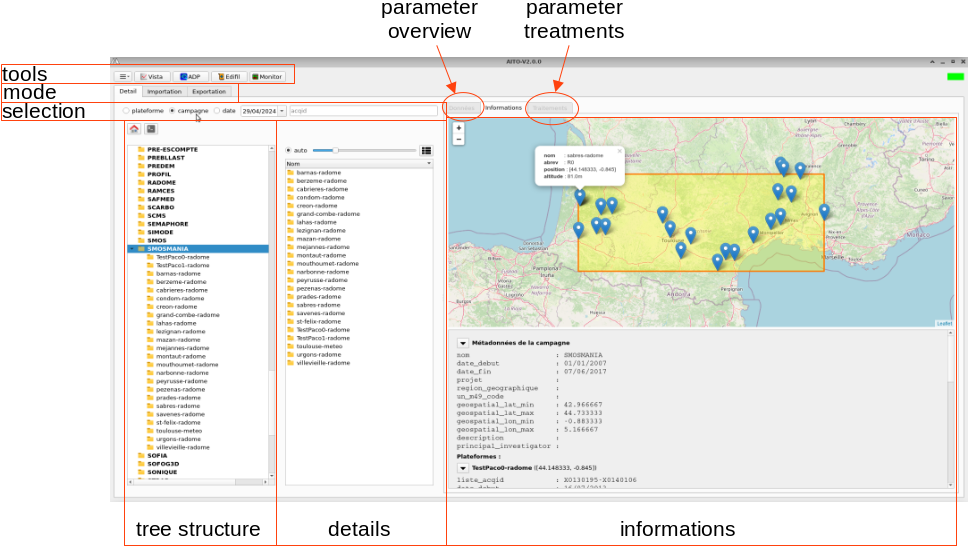
\includegraphics[width=14cm]{images/aito_main.png}
\end{center}

La partie supérieure donne accés, par des boutons, à différents outils de
AIDA (zone \texttt{tools}).

La zone \texttt{mode} permet de visualiser, d'importer et d'exporter des
données.

La zone \texttt{selection} permet de sélectionner le mode de navigation dans
les données (\texttt{plateforme}, \texttt{campagne}, \texttt{date},
\texttt{acqid}). Les zones \texttt{tree structure} et \texttt{detail} sont les
zones d'affichage de la navigation.

La partie droite est constituées de trois onglets (\texttt{information},
\texttt{données}, \texttt{traitements}). L'onglet \texttt{information} permet
de visualiser les informations sur l'objet sélectionné dans la partie
navigation. Lorsqu'un vecteur est sélectionné dans la partie naviagation, les
deux autres onglets (\texttt{données}, \texttt{traitements}) sont activés. \\

L'onglet \texttt{données} affiche les données du vecteur sous formes graphiques,
donne accés à quelques outils et informations concernant le vecteurs.

\begin{center}
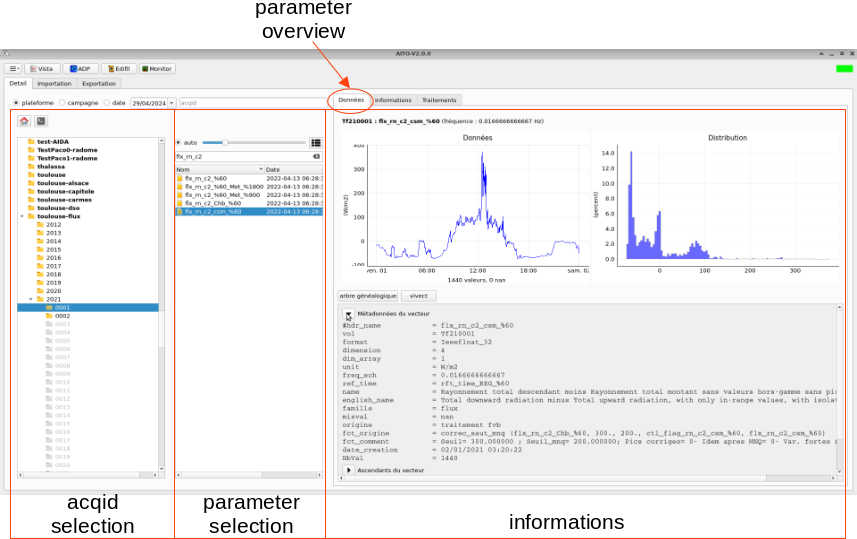
\includegraphics[width=14cm]{images/aito_vecteur_overview.png}
\end{center}

L'onglet \texttt{traitement} permet de visualiser le résultat de quelques
opérateur aux données du vecteur (le résultat des traitement n'est pas
enregistré sur disque).

\begin{center}
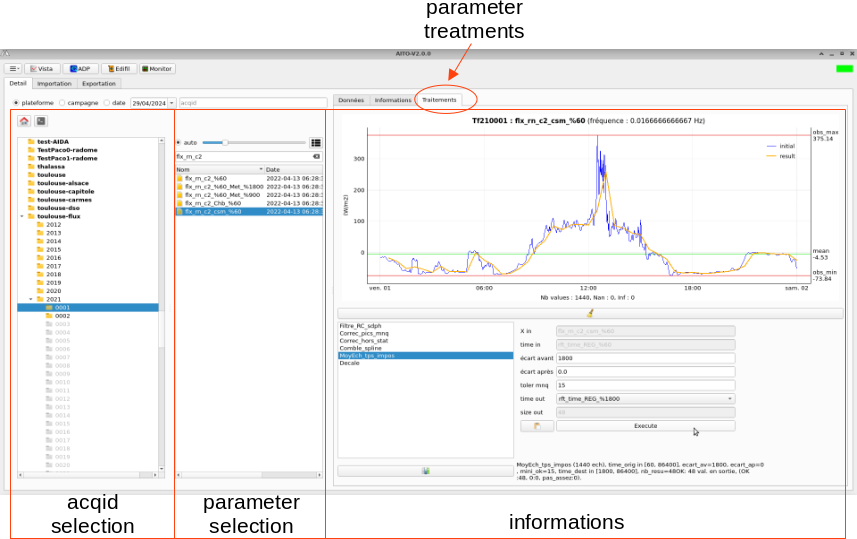
\includegraphics[width=14cm]{images/aito_vecteur_traitement.png}
\end{center}



% Partie 3 : Lecture de fichiers externes
\newpage
\part{Lecture de fichiers externes}
\label{part:lecture}

\section{Introduction}
  Pour stocker les séries de mesure, AIDA utilise son propre format de 
fichiers de données, dit \textit{vecteur}. Les données issues de sources
diverses (en général des systèmes d'acquisition) doivent
donc être converties dans ce format de travail. Pour ce faire, il convient
d'utiliser le programme \texttt{mtv.py} (\textit{miscellaneous to vector})
(page : \pageref{lec-mtv})


\section{Lecture des fichiers d'acquisition : \texttt{mtv.py}}
\label{lec-mtv}
\texttt{mtv.py} permet de convertir des fichiers de données de différents
formats en fichiers-vecteur.

\subsection {Lancement}
\texttt{mtv.py} peut être lancé sous \texttt{aito} (onglet \texttt{Importation})
ou en ligne de commande dans un terminal. \\
Lancer la commande \fbox{ \texttt{mtv.py -h} } pour obtenir de l'aide.

\subsection {Manuel d'utilisation}
\fbox{ \texttt{mtv.py [\textit{options}] <\textit{source}>} }

\medskip
avec :
\begin{itemize}
\item[•] \textit{source} : argument obligatoire. \\
         \textit{source} est :
    \begin{itemize}
      \item \textbf {un fichier} : \\
            toute l'acquition est contenue dans ce seul fichier.
      \item \textbf {liste de fichiers} : \\
            l'acquition est découpée en plusieurs fichiers. La listes des
            fichiers doit être fournie dans l'ordre chronologique de
            l'acquisition.
      \item \textbf {un répertoire} : \\
            le répertoire ne contient que les fichiers des différentes
            parties de l'acquition. \\
            Les fichiers du répertoire sont lus dans l'ordre
            alphabétique : la chronologie de l'acquisition doit donc
            suivre l'ordre alphabétique des fichiers du répertoire.
      \item \textbf {une liste de répertoires} : \\
            la liste des répertoires est lue dans l'ordre fourni. Chaque
            répertoire doit suivre la logique décrite ci-dessus.
    \end{itemize}

\medskip
\item[•] \textit{options} :
    \begin{itemize}
      \item[] \texttt{-a/{}-{}-acqid <acqid>}           : acqid.
      \item[] \texttt{-p/{}-{}-plateforme <plateforme>} : nom long de la plateforme.
      \item[] \texttt{-c/{}-{}-campagne <campagne>}     : nom de la campagne (utile pour renseigner le fichier .inf).
      \item[] \texttt{-f/{}-{}-file <fichier>}          : fichier de configuration (chemin absolu ou relatif).
      \item[] \texttt{-t/{}-{}-type <type>}             : type de fichier à lire (csv\_like, ...).
      \item[] \texttt{-s/{}-{}-start <début>}           : AAAA[MMJJHHMMSS.sss] : date/heure de début des données à lire (inclus).
      \item[] \texttt{-e/{}-{}-end <fin>}               : AAAA[MMJJHHMMSS.sss] : date/heure de fin des données à lire (exclus).
      \item[] \texttt{-n/{}-{}-dry-run}                 : dry run (lecture sans écriture des vecteurs).
      \item[] \texttt{-F/{}-{}-force}                   : écrase les fichiers vecteurs existants.
      \item[] \texttt{-g/{}-{}-graphic}                 : trace les données.
      \item[] \texttt{-C/{}-{}-config <type>}           : aide sur la configuration associée au type de fichier (csv\_like, ...)
      \item[] \texttt{-k/{}-{}-keep}                    : conserve les valeurs hors \textit{[normal\_min, normal\_max]}.
      \item[] \texttt{-L/{}-{}-log\_dir <log\_dir>}     : répertoire des logs (fichier mtv.log).
      \item[] \texttt{-l/{}-{}-logger <logger>}         : fichier de log (chemin complet) dans lequel mtv rajoute ses logs.
      \item[] \texttt{-nc/{}-{}-no-cal}                 : pas de suffixe i\texttt{cal}.
      \item[] \texttt{-nk/{}-{}-no-checksum}            : pas de checksum.
      \item[] \texttt{-r/{}-{}-readers}                 : liste des readers.
      \item[] \texttt{-h/{}-{}-help}                    : affiche l'aide.
    \end{itemize}
\end{itemize}

\medskip
Remarques :

\begin{itemize}
\item la présence d'une des 2 options \texttt{acqid} ou \texttt{plateforme} est obligatoire.
\item si la plateforme est de type acquisition (\texttt{duree\_vecteur} dans le fichier \\
      \texttt{\$AIDA\_HOME/profils/<PROFIL>/plate-formes)} la présence de l'acqid est obligatoire.
\end{itemize}

\subsection {Format du fichier configuration :}
Le fichier de configuration permet à \texttt{mtv.py} de décoder le fichiers
d'acquisition qui peut être des différentes type. Ex :
\begin{itemize}
  \item fichier ASCII avec un en-tête, et des données rangées en colonnes séparées par un ou plusieurs séparateurs).
  \item fichier de type netCDF.
\end{itemize}

\medskip
Liste non exhaustive de fichiers de type ASCII : AROME/ARPEGE, CampbelRAY, G24D1M (Picarro), XSENS, GILL, LI7500, ...

\medskip
Le format du fichier configuration est de type "INI" : il est composé de paragraphes entre crochets suivi d'une liste
d'attributs de type «~champ = valeur~»

\medskip
De manière générale, la colonne est désignée par son numéro \textbf{commençant à 1} ou le nom de colonne définie dans la
ligne de nom de colonne si présente dans l'entête. Cette valeur est désignée :
\ col\_{\textless}\textit{1{\textgreater}} à \ col\textit{\_{\textless}N{\textgreater}} par la suite.

\medskip
Les paragraphes \ [col\_defaut] et [instru\_{\textless}N{\textgreater}] sont optionnels. Ils permettent de définir des
valeurs par défaut des variables. Si les valeurs ne sont pas définies dans le paragraphe de la variable alors les
valeurs des paragraphe [col\_defaut] et [instru\_N] sont utilisées. Cela évite de répéter les informations.

Si on veut utiliser pour un paramètre les valeurs des champs définies dans le paragraphe [instru\_N] alors ajouter un
champ instru = instru\_{\textless}N{\textgreater} dans la description du paramètre.

\medskip
Le paragraphe [msg\_{\textless}ID{\textgreater}] permet de décrire des fichiers où dans un même fichier on trouve des
lignes avec un nombre colonnes et/ou une fréquence des données différentes et dépendant d'une valeur de colonne. 4M
produit couramment ce genre de fichier. Pour les autres types de fichiers les champs définis dans
[msg\_{\textless}ID{\textgreater}] \ doivent être définis dans le paragraphe [structure]

\medskip
{\large \color{blue} [structure] (OBLIGATOIRE)}

\begin{center}
\tablefirsthead{}
\tablehead{\hline champ &
valeur &
Statut &
commentaire\\}
\tabletail{\hline}
\tablelasttail{}
\begin{supertabular}{|p{3.592cm}|p{2.116cm}|p{4.099cm}|p{5.393cm}|}
\hline
champ &
valeur &
Statut &
commentaire\\\hline
nb\_lignes\_entete &
{\itshape nombre} &
Optionnel

défaut = 0 &
Nombre de ligne de l'en{}-tête. \\\hline
numero\_ligne\_nom &
{\itshape nombre ${\geq}$ 1} &
Optionnel

défaut = None &
Numéro de la ligne commençant à 1 contenant les noms des variables correspondant aux colonnes de données. Le séparateur
des noms doit être identique au séparateur de colonnes de données.

Ce système devra être étendu pour traiter des lignes complexes du type : \textit{\textcolor{black}{\#variables : param1,
param2, .{\dots}}}\\\hline
numero\_ligne\_unit &
{\itshape nombre ${\geq}$ 1} &
Optionnel

défaut = None &
Numéro de la ligne contenant les unités des variables correspondant aux colonnes de données. Le séparateur des noms doit
être identique au séparateur de colonnes de données.\\\hline
\textbf{numero\_ligne}

\textbf{\_misval}  

(non implémenté) &
{\itshape nombre ${\geq}$ 1} &
Optionnel

défaut = None &
Numéro de la ligne contenant la valeur de données manquante des variables correspondant aux colonnes de données. Le
séparateur des noms doit être identique au séparateur de colonnes de données.\\\hline
numero\_ligne

\_borne\_inf  &
{\itshape nombre ${\geq}$ 1} &
Optionnel

défaut = None &
Numéro de la ligne contenant les valeurs inférieures des intervalles représentant les bornes des donées 2D. Le
séparateur des bornes doit être identique au séparateur de colonnes de données.\\\hline
numero\_ligne

\_borne\_sup  &
{\itshape nombre ${\geq}$ 1} &
Optionnel

défaut = None &
Numéro de la ligne contenant les valeurs supérieures des intervalles représentant les bornes des donées 2D. Le
séparateur des bornes doit être identique au séparateur de colonnes de données.\\\hline
{\color{black} separateurs\_colonnes} &
{\color{black} \textit{c}\textit{aractère}\textit{\textcolor[rgb]{0.4,0.4,1.0}{ }}\textit{ou \ ESPACE ou TAB}} &
{\color{black} OBLIGATOIRE}

{\color{black} Pas de valeur par défaut.} &
{\color{black} Liste des séparateurs existants dans le fichier de données.}


~

{\itshape\color{black} exemple : ESPACE , ; TAB}

~
\\\hline
{\color{black} separateurs\_multiples}

{\color{black} \_ignores} &
{\color{black} \textit{c}\textit{aractère}\textit{\textcolor[rgb]{0.4,0.4,1.0}{ }}\textit{ou \ ESPACE ou TAB}} &
{\color{black} Optionnel}

{\color{black} défaut = None} &
{\color{black} Séparateurs à ignorer s'ils se succèdent sur la ligne.}

~

{\itshape\color{black} Par exemple : si~ separateurs\_multiples\_ignores= TAB alors plusieurs TAB successifs sur la
ligne seront considérés comme un seul séparateur. }\\\hline
{\bfseries\color{black} separateur\_decimal} 

(non implémenté)&
{\itshape\color{black} caractère} &
{\color{black} Optionnel}

{\color{black} defaut=~'.' (point)} &
~
\\\hline
debut\_ligne\_a\_ignorer &
{\itshape chaîne} &
Optionnel

défaut=None &
Définition d{}'une chaîne de caractères de début de ligne à ignorer par la lecture.\\\hline
colonne\_msg\_id &
{\itshape col\_{\textless}N{\textgreater}}

{\itshape avec N ${\geq}$ 1}

{\itshape ou }

{\itshape col\_{\textless}NOM{\textgreater}}

~

~
 &
Optionnel.

défaut=None

~

Si colonne\_msq\_id n'est pas défini alors on ignore les paragraphes [msg\_{\textless}ID{\textgreater}]

et 

liste\_msg\_id &
~

Numéro de colonne contenant l'identifiant de message pour le cas des fichiers contenant des messages différents
(fréquence et nombre de colonnes).

Si ce champ est renseigné, renseigner les paragraphes [msg\_{\textless}ID1{\textgreater}],
[msg\_{\textless}ID2{\textgreater}], {\dots}.\\\hline
liste\_msg\_id &
\textit{{\textless}ID1{\textgreater}, {\textless}ID2{\textgreater},{\textless}ID3{\textgreater}}

{\itshape (chaîne de caractères)} &
Optionnel mais fortement recommandé dans le cas si colonne\_msg\_id est défini 

défaut = None &
Liste des msg\_ID possibles pour faire du contrôle.\\\hline
traite\_doublons  &
True/False &
Optionnel

défaut = True &
Si True : élimine les données en double (temps et valeur identiques)

Sinon toutes les données sont conservées.\\\hline
ignore\_doublons &
col\_5,col\_8 &
Optionnel

défaut = None &
Liste des colonnes ignorées par la recherche des doublons (séparateur = `,')\\\hline
\end{supertabular}
\end{center}

\medskip
{\itshape\color{black}
Exemple~de fichiers avec plusieurs séparateurs:}

{\itshape\color{black}
18/09/2016 12:00:01.23 CAX1 3.1, 5.2, 7.3}

\medskip
{\itshape\color{black}
separateurs\_colonnes = ESPACE ,}

{\itshape\color{black}
separateurs\_multiples\_ignores= ESPACE}

\medskip
{\texttt{\textbf{\large \color{blue} {[msg\_{\textless}ID{\textgreater}]}}} (existe si colonne\_msg\_id est défini)

\medskip
Si aucun [msg\_{\textless}ID{\textgreater}] n'est défini, les champs ci-dessous \textbf{doivent} se trouver dans le
paragraphe [structure]

\medskip
\begin{center}
\tablefirsthead{}
\tablehead{\hline champ &
valeur &
Statut &
commentaire\\}
\tabletail{\hline}
\tablelasttail{}
\begin{supertabular}{|p{3.504cm}|p{3.7cm}|p{3.642cm}|p{4.448cm}|}
\hline
Champ &
Valeur &
Statut &
Commentaire\\\hline
nb\_colonnes &
{\itshape \ nombre ${\geq}$ 1} &
Optionnel 

{\color{black} Pas utile si numero\_ligne\_nom est défini.}

~

{\color{black} Sinon \ il est OBLIGATOIRE}

~

{\color{black} défaut = None} &
Nombre de colonne de données \\\hline
{\bfseries\color{black} \textmd{temps} }

~

~
 &
{\itshape\color{black} source[d:f],...,source[d:f]

où source peut-être :

col\_{\textless}N{\textgreater}

NOMFIC

NOMREP} &
{\color{black} OBLIGATOIRE}

~
 &
{\color{black} NOMFIC et NOMREP sont des mots clefs.}

{\color{black} d et f représentent les indices de début de et fin de chaîne à décoder (cf. slice python).}

{\color{black} Le séparateur «~,~» est obligatoire et doit se retrouver dans format\_temps. }\\\hline
{\bfseries\color{black} \textmd{format\_temps} } &
{\itshape\color{black} fmt\_1,fmt\_2, ...}

~

{\itshape\color{black} Possibilité de définir plusieurs formats pour un même temps avec le séparateur | :}


{\itshape\color{black} fmt\_1|fmt\_2,fmt\_3,...}  &
{\color{black} OBLIGATOIRE} &
{\color{black} fmt\_1, fmt\_n sont des chaînes de caractères }

{\color{black} décrivant le codage du temps suivant strptime de Python enrichi des formats de délais : }

{\color{black} \%Ds (délai millisecondes),}

{\color{black} \%DS (délai secondes),}

{\color{black} \%DM (delai en minutes),}

{\color{black} \%DH(delai en heures),}

{\color{black} \%Dd(delai en jours),}

{\color{black} ainsi que du format temps GPS : }

{\color{black} \%G(nombre de semaines depuis le 06/01/1980),}


{\color{black} \%Di(secondes intercalaires à enlever)}\\\hline
{\color{black} UTC\_offset} &
{\itshape\color{black} +HHMM} &
{\color{black} Optionnel.}

{\color{black} défaut = +0000} &
{\color{black} UTC Offset (option \%z de strptime) }

~

{\color{black} meta-donnée qui se retrouve dans l'en{}-tête du fichier temps.}\\\hline
{\color{black} nom\_variable\_temps} &
{\itshape\color{black} chaîne } &
{\color{black} Optionnel}

~

{\color{black} défaut = rft\_time\_[nom\_fic config]\_[msg\_ID]} &
{\color{black} Nom du fichier vecteur temps si écriture vecteur , ou nom de variable si renvoi d'une structure de
données.}\\\hline
colonne\_checksum  &
{\itshape col\_{\textless}N{\textgreater} avec N ${\geq}$ 1}

{\itshape ou }

{\itshape col\_{\textless}NOM{\textgreater}} &
Optionnel

défaut = None &
Colonne contenant le check\_sum 

{\itshape ex : col\_7 , col\_CHECK}\\\hline
methode\_check\_sum &
{\itshape\color{black} nom de fonction} &
Optionnel

défaut = None &
Fonction connue de \texttt{mtv.py} avec range comme argument par ex :

{\itshape {\textless}xor\_checksum{\textgreater}:'{\textbackslash}x02', '{\textbackslash}x03'}\\\hline
freq\_ech &
{\itshape\color{black} nombre} &
Optionnel : par défaut la fréquence est calculée à partir des données. &
Fréquence du message en Hz.\\\hline
type\_ech &
{\itshape\color{black} chaîne} &
Optionnel~

défaut = None &
Type d{}'échantillonnage attendu du fichier :

regulier {\textbar} irregulier\\\hline
\end{supertabular}
\end{center}

\medskip
\texttt{\textbf{\large \color{blue} {[col\_defaut]}}} (optionnel)

\medskip
Si les champs ci-dessous ne sont pas définis dans le paragraphe décrivant la colonne alors on prend ces valeurs par
défaut.

\medskip
Les champs autorisés dans ce paragraphe sont :

\begin{itemize}
\item {\bfseries
normal\_min}
\item {\bfseries
normal\_max}
\item {\bfseries
misval\_in}
\item {\bfseries
misval\_out}
\item {\bfseries
invval\_in}
\item {\bfseries
invval\_out}
\item {\bfseries
format}
\item {\bfseries
unit}
\end{itemize}

\medskip
Pour le format de ces champs, voir le paragraphe \ (col\_{\textless}A{\textgreater}) de description des colonnes.

\medskip
\large      \color{blue}\textbf{[\texttt{instru\_N}]}
\normalsize \color{black} (optionnel)

\medskip
Ce paragraphe permet de définir des valeurs de champ liés à un instrument. La prise en compte de ces valeurs pour une
variable se fait via le champ instru= instru\_{\textless}N{\textgreater} dans le paragraphe colonne
(col\_{\textless}A{\textgreater})

\medskip
Les champs autorisés dans ce paragraphe sont :

\begin{itemize}
\item {\bfseries
position}
\item {\bfseries
chaîne acquisition}
\item {\bfseries
module\_{\textless}1{\textgreater} à module\_{\textless}n{\textgreater} }
\end{itemize}

\medskip
Pour le format de ces champs, voir le paragraphe \ (col\_{\textless}A{\textgreater}) de description des colonnes.

\medskip
\large      \color{blue}\textbf{[\texttt{col\_A:\{col\_B\{@msg\_msg\_id\}\}}]}
\normalsize \color{black} (Optionnel)

\medskip
Exemples de nom de paragraphe descriptif de variable :

\medskip
[col\_1] : paramètre de colonne 1

[col\_TPR] : paramètre correspondant à la colonne nommée TPR dans l'en-tête

[col\_2 : col\_10] : paramètre 2D entre les colonnes 2 et 10

[col\_10@msg\_1] : paramètre en colonne 10 pour le msg\_id = 1

\medskip
\begin{center}
\tablefirsthead{}
\tablehead{\hline champ &
valeur &
Statut &
commentaire\\}
\tabletail{\hline}
\tablelasttail{}
\begin{supertabular}{|p{2.9099998cm}|p{3.783cm}|p{4.058cm}|p{4.4500003cm}|}
\hline
{\bfseries\color{black} Champ} &
{\bfseries\color{black} Valeur} &
{\bfseries\color{black} Statut} &
{\bfseries\color{black} Commentaire}\\\hline
ignore  &
{\itshape True/ False} &
Optionnel

défaut = False &
Si 'True' \ la colonne de données correspondante est lue mais la variable n'est pas dans la structure de données
renvoyée (vecteur, ou autre...)\\\hline
{\color{black} controle } &
{\color{black} \textit{{\textless}nom\_fonction{\textgreater}:~{\textless}valeur{\textgreater}}} &
Optionnel

défaut = None &
Permet de spécifier un contrôle sur \ une colonne du fichier. 

Exemples des fonctions implémentées:

{\itshape {\textless}egal{\textgreater} :{}'L751'}\\\hline
instru &
{\itshape instru\_{\textless}N{\textgreater}} &
Optionnel

défaut = None

~

Vérifier que le paragraphe [instru\_{\textless}N{\textgreater}] \ existe. &
Correspond au paragraphe 

instru\_{\textless}N{\textgreater}\\\hline
nom\_variable &
{\itshape chaîne} &
Optionnel

défaut = col\_A ou nom de la colonne &
nom du fichier vecteur si écriture vecteur , ou nom de variable si renvoi d'une structure de données.\\\hline
name &
{\itshape chaîne} &
Optionnel.\newline
défaut = «~col\_A du fichier NOMFIC~» &
Nom long explicite de la variable\\\hline
english\_name &
{\itshape chaîne} &
Optionnel

défaut = «~col\_A from file NOMFIC~» &
Nom long explicite en anglais de la variable\\\hline
unit &
{\itshape chaîne} &
Optionnel mais fortement recommandé.

défaut = unknown &
Unité de la variable après application de la «~law~» éventuelle, \ acceptable par libudunits2\\\hline
format  &
{\itshape chaîne} &
Optionnel

défaut=ieeefloat32 &
Format connu de AIDA\\\hline
law &
{\itshape chaîne} &
Optionnel.

defaut = None &
Loi à appliquer selon norme AIDA 
(voir doc package readers,
 
module abstract\_reader,
 
rechercher 'law')

Si pas de law écriture directe d'un vecteur « cal »

Si présence de law écriture du vecteur BRUT « raw » et du vecteur « cal »

~

~
\\\hline
normal\_min &
{\itshape nombre} &
Optionnel

defaut=None &
Borne min de l'intervalle de validité de la variable (après application d'une éventuelle law).\\\hline
normal\_max &
{\itshape nombre} &
Optionnel

defaut=None &
Borne max de l'intervalle de validité de la variable (après application d'une éventuelle law).\\\hline
misval\_in &
{\itshape chaîne} &
Optionnel

défaut = NULL &
Valeur manquante dans le fichier d'entrée.

Si non NULL la présence d'un champ vide doit générer un signalement.\\\hline
misval\_out &
{\itshape chaîne} &
Optionnel

défaut = NaN &
Valeur manquante dans les données de sortie.\\\hline
invval\_in &
{\itshape chaîne} &
Optionnel

défaut = NULL &
Valeur invalide (différente de misval\_in) dans le fichier d'entrée\\\hline
invval\_out &
{\itshape chaîne} &
Optionnel

défaut = misval\_out &
Valeur invalide dans le tableau ou vecteur produit (champ invval du fichier vecteur)\\\hline
bornes  &
{\itshape (x{1} ,y{1} ); ...; (x{n },y{n} )}

(cf documentation de référence)

ou

{\itshape auto}&
Optionnel mais fortement recommandé si la variable est un tableau 1D

défaut = None &
Ce champ précise les bornes de chacun des éléments du tableau. S'il vaut auto, les valeurs des bornes sont automatiquement lues dans le fichier de données en utilisant les champs numero\_ligne\_borne\_inf et numero\_ligne\_borne\_sup.\\\hline
unit\_bornes &
{\itshape chaîne} &
Optionnel mais fortement recommandé

défaut = None &
Indique l'unité de l'attribut bornes\\\hline
position &
{\itshape chaîne} &
Optionnel mais fortement recommandé !

défaut = None &
Position de la mesure\\\hline
orientation &
{\itshape chaîne} &
Optionnel

défaut = None &
Lorsque le paramètre contenu dans un vecteur est une grandeur physique orientée

(un angle, une distance sur un axe, une composante d'un vecteur), ce champ contient une

description de cette orientation\\\hline
chaîne\_acquisition &
\textit{module\_1 {\dots}. module\_n} &
Optionnel mais fortement recommandé !

défaut = None &
Description de la chaîne d'acquisition selon norme AIDA (liste des modules)\\\hline
module\_{\textless}1{\textgreater} à module\_{\textless}n{\textgreater} &
{\itshape {\textless}type\_module{\textgreater}:{\textless}fabricant{\textgreater}:{\textless}Modèle{\textgreater}
:{\textless}Numéro de série{\textgreater}:{\textless}Numéro de référence}

{\itshape interne{\textgreater}:{\textless}date et lieu de calibrage ou étalonnage{\textgreater}} &
Optionnel mais fortement recommandé !

défaut = None &
Description d{}'un module d'acquisition selon norme AIDA\\\hline
information &
{\itshape chaîne } &
Optionnel

défaut = None &
Commentaire libre\\\hline
\end{supertabular}
\end{center}

\medskip
{\color{black}
Il est possible d'ajouter des champs à cette liste mais ils ne seront pas écrits dans les vecteurs. Ils seront dans la
structure de données renvoyée.}

\medskip
Les champs suivants sont présents dans les vecteurs produits mais déterminés automatiquement :

\medskip
\begin{itemize}
\item \textbf{dim\_array}~: est déterminé \ à partir de la dimension de chaque variable 
\item \textbf{obs\_min }et \textbf{obs\_max}~: sont calculées automatiquement
\item \textbf{freq\_ech} : calculée à partir du \ temps lu (inverse de la médiane de \texttt{${\Delta}$}t)
\item \textbf{famille}\textbf{~}: déterminée à partir des 3 premières lettres du champ \textbf{nom\_variable}
\item \textbf{origine~ }vaut «~lecture~»
\item \textbf{fct\_origine : }est la copie de la commande mtv complète~: «~ mtv {\dots}.~»
\end{itemize}

%%%\medskip
%%%\begin{itemize}
%%%\item[] 
%%%\bigskip
%%%\end{itemize}

\subsection{Evolution des fichiers de configuration dans le temps}
\label{sec:histo_config}
\texttt{mtv.py} ne prend pas en charge la gestion de l'évolution des fichiers
de configuration au cours du temps. Cela doit être fait en amont. AIDA dispose de
l'outil \texttt{histo\_config.py}. Cet outil utilise des fichiers .histo et
permet de connaître le fichier de configuration à utiliser par mtv en fonction de la
date.

\medskip
\subsubsection{Format des fichiers .histo}
Les fichiers .histo sont des fichiers de type .ini contenant des {\bfseries [sections]} et des lignes de type {\bfseries attribut = valeur} où :

{\bfseries section} = coupleur

{\bfseries attribut} = intervalle de temps => YYYY-mm-ddTHH:MM:SS~~YYYY-mm-ddTHH:MM:SS

{\bfseries valeur} = fichier de configuration utilisé par mtv

\subsubsection{Exemple de fichier .histo}
\# METEOPOLE-FLUX

\# Historique des fichiers configuration de la plateforme toulouse-flux

\#

\#

[campbel1]

2012-06-15T00:00:00 2015-06-20T23:59:59 = METEOPOLE\_FLUX.toulouse-flux.campbel1.V0.config

\# ajout du KT15

2015-06-21T00:00:00 2030-12-31T23:59:59 = METEOPOLE\_FLUX.toulouse-flux.campbel1.V1.config



[campbel2]

2012-06-15T00:00:00 2016-01-20T23:59:59 = METEOPOLE\_FLUX.toulouse-flux.campbel2.V0.config

\# ajout de la ventilation du CNR1

2016-01-21T00:00:00 2030-12-31T23:59:59 = METEOPOLE\_FLUX.toulouse-flux.campbel2.V1.config



[campbel3]

2012-06-15T00:00:00 2030-12-31T23:59:59 = METEOPOLE\_FLUX.toulouse-flux.campbel3.V0.config



\subsection{Gestion des «~log~»}
Le programme mtv.py écrit ses logs aux moyen du module python loggin.

Plusieurs loggers sont utilisés :

\begin{itemize}
\item mtv.log : ce fichier est systématiquement créé avec le niveau DEBUG. Par défaut, il se trouve sous /tmp mais son
emplacement peut être défini par l'option {}-L/-{}-log\_dir. Le fichier mtv.log est un logger de type
RotatingFileHandler~: dès que le fichier atteint une taille de 100Mo il est renommé et un autre fichier se crée. On
conserve ainsi une archive de 10 fichiers en mode tournant.
\item stdout : l'écriture sur stdout se fait en mode INFO par défaut. La variable d'environnement MTV\_LEVEL (DEBUG
{\textbar} INFO {\textbar} WARNING {\textbar} ERROR) permet de modifier le niveau de log
\item l'utilisateur peut également spécifier un fichier de log via l'option -l/-{}-logger dans lequel mtv ajoutera ses
logs en mode DEBUG.
\end{itemize}

\subsection[Architecture ]{Architecture} 
Le package «~readers~» contient les fonctions de «~lecture données~» et
«~contrôle temps~». Il est appelable par n'importe quel programme Python.
Il n'est pas spécifique ni de AIDA ni du format vecteur. Pour plus de
commodité nous installons néanmoins ce package dans AIDA.

\medskip
\texttt{mtv.py} est basé sur le package de lecture de données «~readers~».

\medskip
«~readers~» se trouve sous \texttt{\$AIDA\_HOME/src/python3/packages/readers}

\medskip
\texttt{mtv.py} se trouve sous \texttt{\$AIDA\_HOME/src/python3/lecture/mtv}

\clearpage
\subsection[Exemples de description du temps]{Exemples de description du temps dans le fichier configuration}
\tiny
\begin{flushleft}
\tablefirsthead{}
\tablehead{\normalsize\hline
{\bfseries Type de fichier} &
{\bfseries Format de la datation} &
{\bfseries Description dans fichier configuration }\\\tiny}
\tabletail{\hline}
\tablelasttail{}
\begin{supertabular}{|p{4.109cm}|p{5.3cm}|p{6.284cm}|}
\hline
{\bfseries \normalsize Type de fichier} &
{\bfseries \normalsize Format de la datation} &
{\bfseries \normalsize Description dans fichier configuration }\\\hline
AROME/ARPEGE &
2016050113 12.43 {\dots}.  &
separateur\_colonnes = ESPACE

temps = col\_1

format\_temps =\%Y\%m\%d\%H\\\hline
Fichier Campbel 4M (avant MEF)  &
17/05/2016 00:00:00.060 CMI1 {\textquotedbl}05/17/2016 00:00:00{\textquotedbl} , {\dots}.

~
 &
separateur\_colonnes = ,

temps = col\_1[0:23]

format\_temps =\%d/\%m/\%Y \%H:\%M:\%S.\textcolor{black}{\%f}\textcolor{red}{ }

(respecter l'espace entre date et heure dans \ 

format\_temps)\\\hline
Fichier GILLV 4M  &
\ 31/05/2016 00:30:00.022 GIV1 220 9 56 17049  &
separateur\_colonnes = ESPACE

temps = col\_1, col\_2

format\_temps=\%d/\%m/\%Y,

\%H:\%M:\%S.\textcolor{black}{\%f }\\\hline
Fichier GILL et XSENS nacelle turbulente &
Nom de fichier : tr\_09080842.GIL ou tr\_09080842.XSE

Dans les fichiers :

~

08:08:42.261,3, {\dots}. &
On n'a pas la date complète ni dans le nom du fichier, ni dans les données. Passer l'Acqid en argument de \texttt{mtv.py}

~

Dans le fichier configuration on aura :

separateur\_colonnes = ,

temps = col\_1

format\_temps = \%H:\%M:\%S.\textcolor{black}{\%f}\textcolor{red}{ }

~

{\color{black} \textbf{ou} si on a la date complète dans nom de fichier (Eric peut nous faire ça ..)}

{\color{black} comme par exemple : \ tr\_2016\_09080842.GIL}

~

{\color{black} separateur\_colonnes = ,}

{\color{black} temps = NOMFIC[3:12], col\_1}

{\color{black} format\_temps =\%Y\_\%m\%d, \%H:\%M:\%S.\%f }

~
\\\hline
Essais KH20~(4M): &
Dans les fichiers :

{\textquotedbl}2015-07-02 12:59:14.9{\textquotedbl},382355,{\dots}..

{\textquotedbl}2015-07-02 12:59:15{\textquotedbl},382356, {\dots}.. &
separateur\_colonnes = ,

temps = col\_1

format\_temps =~'{}'\%Y-\%m{}-\%d\%H:\%M:\%S.\%f'{}'

~

Attention parfois on n'a pas les décimales ...\\\hline
RADOME vidage Degreanne &
20141029000600 70 2.4 &
separateur\_colonnes = ESPACE

temps = col\_1

format\_temps =\%Y\%m\%d\%H\%M\%S\\\hline
PICARRO  &
DATE \ \ \ \ \ \ \ \ \ \ \ \ TIME \ \ \ \ \ \ \ \ FRAC\_DAYS\_SINCE\_JAN1

2015-11-05 \ \ \ \ 13:04:00.000 \ 308.54444444 &
separateur\_colonnes = \ ESPACE

temps = col\_DATE,col\_TIME

format\_temps =\%Y-\%M{}-\%d,\%H :\%M :\%S\\\hline
Message AIPOV de l'AIRINS &
\$AIPOV,133306.6012,...

\$AIPOV,133306.6112,... &
separateur\_colonnes = ,

temps = col\_2

format\_temps =\%H\%M\%S.\%f\\\hline
Températures de brillance issues de rad2Tb  &
2013-05-30,07:54:01.392, 7.90039,284.696...

2013-05-30,07:54:01.552, 7.90043,284.714...

2013-05-30,07:54:01.712, ... &
separateur\_colonnes = ,

temps = col\_Date,col\_ClockTime

format\_temps =\%Y-\%m-\%d,\%H :\%M :\%S.f \\\hline
PACS &
1,\#2014-03-26 13:31:06\#,633,\#2014-03-26 13:31:06\#,633,1000 &
separateur\_colonnes = ,

temps = col\_2

format\_temps= \#\%Y-\%m-\%d \%H :\%M :\%S\#\\\hline
Licor7500 &
DATAH\ \ Time\ \ Date\ \ Sequence Number 

DATA\ \ 04:39:30:549\ \ 2012-09-26\ \ 298870 &
separateur\_colonnes = TAB

temps = col\_Date,col\_Time

format\_temps =\%Y-\%m-\%d,\%H :\%M :\%S

~
\\\hline
RS format \ 

RS\_FLEDT\_G4253301\_

20121031085852.tsv

~

~
 &
time Pscl T RH v u ...

0000 28372.5 291.85 81 1.84228 3.32355 2 ...

0002 28368.4 291.666 85.172 1.85628 2.9116 ... &
separateur\_colonnes = ESPACE

temps = NOMFIC~[18:32], col\_time

format\_temps =\%Y\%m\%d\%H\%M\%S,\%Ds\\\hline
\end{supertabular}
\end{flushleft}
\normalsize

\subsection{Fichier d'acquisition au format netCDF}
\fbox{ \texttt{mtv.py -C netcdf} } \\
permet d'obtenir de l'aide sur la structure du fichier de configuration attendu
par le reader \texttt{netcdf}.


% Partie 4 : Traitements
\newpage
\part{Traitements, calculs}
\label{part:traite}

\section{L'interpréteur de commandes : \texttt{adc}}

  Le système de traitement d'AIDA est construit autour d'un
langage de commande, qui permet d'exécuter des fonctions
de traitement sur des données choisies.

\medbreak
\textbf{\textit{Note : adc est le résultat de la réécriture en langage Python
de l'interpréteur de commande initial (écrit en langage C) : fvb}}

\subsection{Le langage}

Une ligne de commande doit avoir la forme suivante :

\fbox{ \texttt {opérateur ( argument [, autre\_argument] )} }

\medbreak
Une ligne de commentaire commençe par \texttt{\#} :

\fbox{ \texttt{\# commentaire }} \\

\bigbreak
On appelle \texttt{opérateur} une fonction de calcul qui a deux
particularités :
\begin{itemize}
  \item d'une part, cette fonction travaille sur l'ensemble de la série
        temporelle de mesure,
  \item d'autre part, elle est décrite de façon plus complète qu'une fonction
        d'un langage de programmation classique, ce qui permet au système de
        mieux vérifier les arguments en entrée, et de mieux renseigner les
        attributs des résultats (en particulier pour leur unité).
\end{itemize}

\medbreak
L'ensemble des opérateurs disponibles est documenté dans le catalogue : \\
\texttt{\$AIDA\_HOME/doc/CATALOG\_OPER.pdf}.

\medbreak
Les arguments peuvent être :
\begin {itemize}
  \item le nom d'une série de mesure (nom du ``vecteur'', pas du fichier)
  \item un nombre
  \item une constante symbolique de la liste ci-dessous
        (voir : \ref{sec:Cste}, page \pageref{sec:Cste}).
  \item une référence à un attribut de l'acquisition. \\
        La syntaxe est alors : \\
        \texttt{\$Acq.<nom\_rubrique>.<nom\_attribut>}
        (voir : \ref{sec:Acq}, page \pageref{sec:Acq}).
  \item une référence à un attribut d'un argument précédent. \\
        La syntaxe est alors : \\
        \texttt{\$Arg\textit{xx}.nom\_attribut}
        (voir : \ref{sec:Arg}, page \pageref{sec:Arg}).
  \item une valeur de paramètre qui évolue dans le temps. \\
        La syntaxe est alors : \\
        \texttt{\$Chrono.PARAM}
        (voir : \ref{sec:Chrono}, page \pageref{sec:Chrono}).
  \item une formule utilisant un nombre, une constante ou un attribut. \\
        Les opérations connues sont : +-*/
  \item un paramètre optionnel de l'opérateur
        (voir : \ref{sec:param_opt_oper}, page \pageref{sec:param_opt_oper}).
  \item un paramètre optionnel de \texttt{adc}.
        (voir : \ref{sec:param_opt_adc}, page \pageref{sec:param_opt_adc}).
\end {itemize}

\subsubsection{Les constantes symboliques}
  Elles sont définies dans le fichier : \\
\-\hspace{1cm} \texttt{\$AIDA\_HOME/src/python3/AIDA\_lib/Constantes.py}. \\
Les \textit{constantes simples} sont les suivantes :

\label{sec:Cste}
\begin{tabular}{l|l|l}
 nom          & type       & valeur \\
\hline
 ieeefloat64\_max & double  & 1.7976931348623157e+308 \\
 ieeefloat32\_max & float  & 3.40282347e+38 \\
 int32\_max    & int\_32  & 2147483647 \\
 int16\_max    & int\_16  & 32767 \\
 pi           & double  & 3.14159265358979323846 \\
 DegRad       & double  & 3.14159265358979323846 / 180.0 \\
 RadDeg       & double  & 180.0 / 3.14159265358979323846 \\
 KtMs         & double  & 1852.0 / 3600.0 \\
 FtmMs        & double  & 0.3048 / 60.0 \\
 FtM          & double  & 0.3048 \\
 g            & double  & 9.806650 \\
 T0           & double  & 273.15 \\
 sigma        & double  & 5.67051e-8 \\
 sigma\_LOA    & double  & 5.6698e-8 \\
 R            & double  & 8.314510 \\
 Ra           & double  & 8.314510 / 0.028964 \\
 Rv           & double  & 461.51 \\
 cpa          & double  & 1004.685 \\
 cva          & double  & 717.64 \\
\end{tabular}

\medbreak
  Se référer directement au fichier des constantes pour les valeurs des
\textit{constantes plus compliquées} :
\begin{verbatim}
- SA_PMS_OAP230Y
- SA_PMS_OAP200X_INSU
- SA_PMS_OAP200X_LaMP
- FSSP300_std_mid_diam
- SPP200_std_mid_diam
- PCASP_std_mid_diam
- GRIMM1_109_std_mid_diam
\end{verbatim}

\subsubsection{Les attributs de l'acquisition \$Acq}
\label{sec:Acq}
  La syntaxe générale est : \\
\texttt{\$Acq.<nom\_rubrique>.<nom\_attribut>}

\medbreak
  Les dates sont des quantités qui peuvent être exprimées de plusieurs manières,
une syntaxe spécifique a donc été mise en place. La forme générale est : \\
\texttt{\$Acq.\$nom\_de\_la\_date.quantité}.

\bigbreak
Actuellement, la seule syntaxe utilisable est : \\
\fbox{ \texttt{\$Acq.\$date.DOY} } \\
qui donne la date d'acquisition (champ \texttt{date} de la rubrique
\texttt{[IDENTIFICATION]} du fichier .inf), exprimée sous la forme d'un numéro
du jour dans l'année.


\subsubsection{Les attributs des arguments \$Arg}
\label{sec:Arg}
Les noms des attributs des arguments correspondent
généralement aux noms des champs de l'en-tête des
fichiers vecteurs, à quelques exceptions près, soit
pour des raisons historiques (sample, array\_dim), soit
pour désigner une information qui n'existe pas
dans l'en-tête (NbVal).

\begin{tabular}{r l}
 \textbf{Nom}          & \textbf{Signification}  \\
\hline
 nom & le nom du vecteur (chaîne de caractère)\\
 array\_dim & la dimension de chaque échantillon (nombre)\\
 array\_shape & dimensions (au sens shape) des données (chaîne de caractère)\\
 sample & la fréquence d'échantillonnage (nombre)\\
 NbVal & le nombre d'échantillons (nombre)\\
 unit & l'unité (chaîne de caractère) \\
 time\_bnds & bornes temps (chaîne de caractère)\\
 misval & la valeur manquante (même type que le vecteur) \\
 famille & la famille du paramètre (chaîne de caractère ) \\
 name & le nom long (chaîne de caractère ) \\
 english\_name & le nom long en anglais (chaîne de caractère ) \\
\end{tabular}

\subsubsection{Les attributs \$Chrono}
\label{sec:Chrono}
Les attributs de type \$Chrono.PARAM permettent de gérer des paramètres de
traitement qui évoluent avec le temps. La valeur de PARAM est lue dans un
fichier de configuration associé à la plateforme dans lequel sont décrites
les valeurs que prend PARAM en fonction de la date. Ce fichier est décrit
dans le document de référence volume 1 : \url{refman.pdf}.

\subsubsection{Les paramètres optionnels de l'opérateur}
\label{sec:param_opt_oper}
Certains opérateurs peuvent accepter des arguments optionnels.
Ceux-ci sont présentés dans la documentation de l'opérateur sous la rubrique :
\textbf {Entrées optionnelles}.

La forme générale pour fournir un argument optionnel dans la ligne de commande
est : \fbox{ \texttt {<argument>=<valeur>} }
\medbreak

La forme de la valeur de l'argument optionnel dépend du type de l'argument
définit dans la documentation de l'opérateur:

\begin{itemize}
  \item[•] \texttt{NUM}    : l'argument attendu est un numérique (entier,
                             flottant, etc). \\
                             Ex : \texttt{value=12}

  \item[•] \texttt{list()} : l'argument attendu est une liste python. \\
                             Ex : \texttt{value=[0, 100]}

  \item[•] \texttt{dict()} : l'argument attendu est un dictionnaire python. \\
                             Ex : \texttt{value=\{"min"=0, "max"=100]\}}

  \item[•] \texttt{bool()} : l'argument attendu est un booléen python
                             (True, False). \\
                             Ex : \texttt{value=True}

  \item[•] \texttt{str()}  : l'argument attendu est une chaîne python \\
                             Ex : \texttt{value="radian"}

\end{itemize}

\subsubsection{Les paramètres optionnels de adc}
\label{sec:param_opt_adc}

Ces paramètres sont traités directement par \texttt{adc} (on peut donner
autant de paramètres de type que nécessaire).

Ils permettent de remplacer la valeur d'un champ du header des vecteurs de
sortie par une valeur définie par l'utilisateur. \\
Ils permettent également de créer un champ dans le header des vecteurs de
sortie.
\medbreak

La forme générale pour fournir un argument optionnel de \texttt{adc} dans la
ligne de commande est : \fbox{ \texttt{HDR\_xxx=[..., ...]} }
\medbreak
  où : \texttt{xxx} est le nom d'un champ du header du vecteur de sortie
  existant ou \textbf{à créer} (Ex : \texttt{HDR\_english\_name},
  \texttt{HDR\_SPECIAL\_comment}).
\medbreak

La partie entre crochets (\texttt{[]}) doit contenir autant de valeurs
de remplacement que de vecteurs de sortie de l'opérateur, séparées par des
virgules (\texttt{','}). \\
Si pour un vecteur de sortie \texttt{adc} ne doit par modifier la valeur
positionnée par l'opérateur, sa valeur doit être : \texttt{None}. \\
\medbreak

Exemple : pour un opérateur qui génère 3 vecteurs de sortie, si l'appel de
l'opérateur contient : \\
\textbf{\texttt{ HDR\_english\_name=['new name for param x', None, 'new name for param z']}} \\
alors : \\
\begin{itemize}
  \item[•] le vecteur de sortie n°1 contiendra :
	       \texttt{english\_name = new name for param x}
  \item[•] le vecteur de sortie n°2 contiendra :
           \texttt{english\_name = <l'english\_name calculé par l'opérateur>}
  \item[•] le vecteur de sortie n°3 contiendra :
           \texttt{english\_name = new name for param z}
\end{itemize}
\medbreak

Exemple : pour un opérateur qui génère 1 vecteur de sortie, si l'appel de
l'opérateur contient : \\
\textbf{\texttt{ HDR\_SPECIAL\_comment=['commentaire'] }} \\
alors : \\
\begin{itemize}
  \item[•] le vecteur de sortie contiendra : \texttt{SPECIAL\_comment = commentaire}
\end{itemize}
\medbreak


\subsection{Exemples}

\textbf{\textit{Note : l'écriture de fichier de commande pour adc (.fil) est
grandement facilitée par l'utilisation de l'interface graphique \texttt{edifil}
(voir \nameref{sec:edifile})}}

\subsubsection{Exemple d'appel d'un opérateur}

La ligne de commande pour calculer la somme de deux vecteurs (qui doivent
être synchrones, bien sûr) est : \\
\texttt{Plus (<nom\_premier\_vect>, <nom\_second\_vect>, <nom\_résultat>)}

\subsubsection{Exemple de fichier de commandes de traitement (.fil)}
\newgeometry{margin=1cm}
\begin{landscape}
\thispagestyle{mylandscape} %Call our predefined page type
  \begin{lstlisting}
    # Traitement des donnees pluvio
    # - Calculs de précipitation de la station meteopole-flux
    
    # Quantité de précipitation sur 1 mn
    # (pluvio de reference de la DSO reférencé dans le fichier chrono)
    Ech_tps_impos ($Chrono.CHOIX_PLUVIO, $Chrono.REFTIME_PLUVIO, 60., rft_time_REG_%60, $Arg4.NbVal, prp_rr_min_c2_Eti_%60) 
    
    # On effectue un remplissage avec des valeurs nulles pour le flag = 2
    Remplace_selon_flag (prp_rr_min_c2_Eti_%60, ctl_flag_invalid_pluvio_%60, 1.9, 2.1, 0, prp_rr_min_c2_remplac_%60)
    
    # On interpole pour eviter la valeur manquante sur la derniere minute
    Correc_hors_bornes (prp_rr_min_c2_remplac_%60, 0.,100.,1,$Arg1.misval, prp_rr_min_c2_Chb_%60)
    Poly_1_flt (prp_rr_min_c2_Chb_%60,0.,1.0, "mm" , "", "", prp_rr_min_c2_mm_%60) 
    
    # Cumul des quantités de precipitation sur 1 heure
    Som(prp_rr_min_c2_mm_%60,60,0, prp_rr_cumul_%60_%3600)
    
    # Calcul de la série quotidienne de cumul de RR
    Cumul (prp_rr_min_c2_Chb_%60, prp_rr_auto_cumule_%60)
  \end{lstlisting}
\end{landscape}
\restoregeometry


\subsection{Lancement}
\texttt{adc} peut être lancé sous \texttt{aito} par l'intermédiaire de l'outil
\texttt{edifil} (bouton \texttt{edifil})
ou en ligne de commande dans un terminal :

\fbox{ \texttt{adc  [options] acqids [Fichier\_de\_commandes\_de\_traitement]} }

\medbreak
avec : \\
\begin{itemize}
  \item[•] \texttt{acqids} : un identificateur d'acquisition unique
    \textbf{ou} une séquence d'identificateurs. Dans ce dernier cas, la
    forme est : \texttt{<premier\_acqid>-<dernier\_acqid>}. \\
    Ex :
    \begin{itemize}
      \item as200015 : le traiement sera appliqué à la seule acquisition as200015.
      \item as200015-as200019 : le traiement sera appliqué à toutes les
            acquisitions comprises entre [as200015, as200019].
    \end{itemize}

  \item[•] \texttt{[Fichier\_de\_commandes\_de\_traitement]} : fichier
    contenant les commandes adc à appliquer à \texttt{acqids}.
    Usuellement, l'extension du nom de ce type de fichier est
    \texttt{\textbf{.fil}}. \\
    Si cet argument optionnel n'est pas donné, les commandes sont lues sur
    l'entrée standard.

  \item[•] Sans option : le résultat est écrit sur disque si
    le vecteur n'existe pas.

  \item[•] Les options possibles sont les suivantes :
    \begin{description}
      \item -h : affiche un court texte d'aide.

      \item -v : affiche des informations de version.

      \item -V : mode \textit{Verbose}. Augmente le niveau des traces écran.

      \item -S : mode \textit{stop on error}.  Arrêt de adc à la première
                 erreur rencontrée. \textit{Défaut} : False

      \item -M <mail-list> : mode \textit{mail-to}. Le fichier de
                 configuration \\
                 \texttt{\$AIDA\_HOME/profils/\$AIDA\_PROFIL/AIDA\_mail.cfg}
                 doit exister (voir : \ref{ex:mail}, page \pageref{ex:mail}).
                 Les adresses sont séparées par des virgules (,) sans espaces.

      \item -f : mode \textit{versionning}. Les résultats sont toujours écrits
                 sur disque/base, en créant éventuellement une version de
                 sauvegarde (\texttt{<paramètre>.vx.vbn}) d'un paramètre de
                 même nom déjà existant.

      \item -F : mode \textit{force}. Les résultats sont toujours écrits sur
                 disque/base, en remplaçant éventuellement un paramètre de
                 même nom déjà existant.

      \item -N<i> : mode \textit{développement}. Les résultats sont toujours
                    écrits sur disque, une version n<i> est créée
                    (\texttt{<paramètre>.n<i>.vbn}).

      \item -C : invalide le contrôle sur les familles.
                 Cette option permet de retraiter les anciennes acquisitions
                 comme le faisait fvb (qui ne faisait pas ce contrôle)

      \item -T : mode \textit{test et validation}. Avant d'écraser un vecteur
                 xxx.vbn, généré par fvb, adc le renomme xxx.FVB.vbn. Ce
                 vecteur pourra, par la suite, être utilisé par l'outillage de
                 validation du répertoire :
                 \path{src/python3/packages/AIDAcalc/validation}.
    \end{description}
\end{itemize}


\subsubsection{Exemple de fichier de configuration des mails automatiques}
 \label{ex:mail}
 \begin{lstlisting}
  # configuration pour les mails automatiques
  [AIDAcalc]
  smtp      = smtp.xxx.yyy
  from_addr = aaa.bbb@domaine
 \end{lstlisting}


\section{IHM graphique de adc : \texttt{edifil}}
\label{sec:edifile}
L'interface graphique \texttt{edifil} permet d'écrire des fichiers de
commandes pour l'interpréteur de commande \texttt{adc} (fichiers \texttt{.fil}
décrits ci-dessus). \texttt{edifil} permet également de tester ou exécuter
les fichiers \texttt{.fil} sur un \texttt{acqid}.

\subsection{Lancement}
\texttt{edifil} peut être lancé sous \texttt{aito} (bouton \texttt{edifil})
ou en ligne de commande dans un terminal :

\fbox{ \texttt{edifil.py [\textit{options}] [\textit{file ...}]} }

\medskip

avec :

\begin{itemize}
\item[•] \textit{options} :
    \begin{itemize}
      \item[] \texttt{-h/{}-{}-help}                    : affiche l'aide.
    \end{itemize}

\item[•] \textit{file ...} : argument facultatif. Un ou plusieurs fichiers de
                             commandes pour adc (.fil)
\end{itemize}

\medskip


\subsection{Présentation}
La page principale de \texttt{edifil} comporte plusieurs parties :

\begin{center}
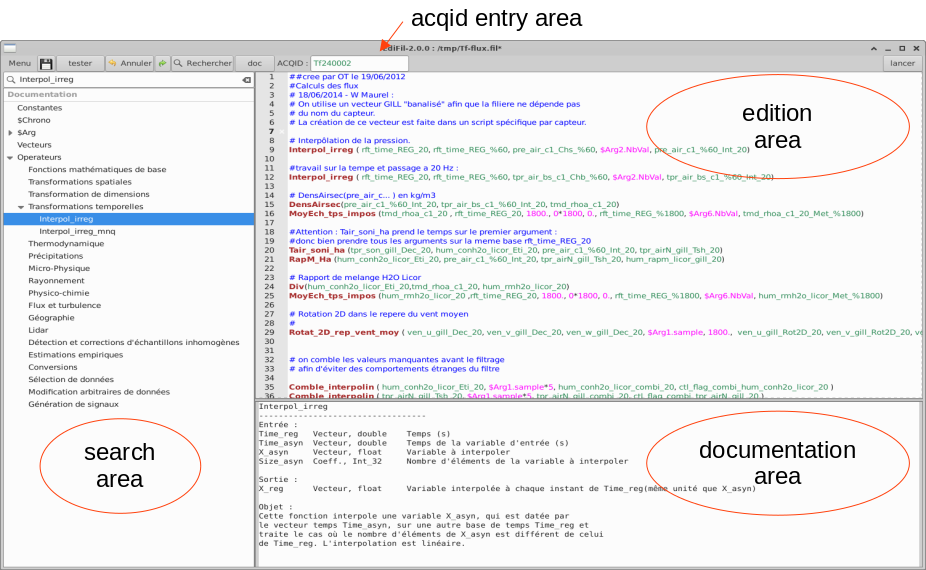
\includegraphics[width=14cm]{images/edifil.png}
\end{center}

L'aide de \texttt{edifil} est présentée sous l'entrée \textbf{Aide du Menu}.


% Partie 5 :  Production de graphiques
\newpage
\part{Production de graphiques}

\label{part:graphe}
\section{Introduction}
Il existe sous AIDA plusieurs outils de production de graphiques qui seront
décrits dans la suite de cette partie.

\begin{itemize}
    \item[•] \texttt{adp}             : visualisation des données d'une
                                        acquisition.
    \item[•] \texttt{vista}           : visualisation des données d'acquisitions
                                        sur toute une période.
    \item[•] \texttt{gengraphvect.py} : graphe de généalogie d'un vecteur.
    \item[•] \texttt{genparamvect.py} : graphe de généalogie d'un vecteur avec
                                        suivi d'un paramètre du header.
\end{itemize}

Ces outils peuvent être lancés en mode non-interactif ("\textit{mode batch}")
afin de produire des fichiers Quicklooks.
La génération automatique des fichiers Quicklook peut être faite
par la commande système \texttt{cron}.


\section{\texttt{adp} et son compagnon \texttt{adpbatch}}
\texttt{adp} (AIDA plot) permet de visualiser graphiquement les données d'une
acquisition.
Il permet également de créer un fichier de configuration qui pourra être
utilisé par son compagnon \texttt{adpbatch} pour générer des fichiers
Quicklooks en mode non-interactif ("\textit{mode batch}").

\subsection{Lancement}
\texttt{adp} peut être lancé sous \texttt{aito} par l'intermédiaire du bouton
\texttt{adp}
ou en ligne de commande dans un terminal. \\
Lancer la commande \fbox{ \texttt{adp -h} } pour obtenir de l'aide.

\subsection{Présentation}
La page principale de \texttt{adp} comporte plusieurs parties :

\begin{center}
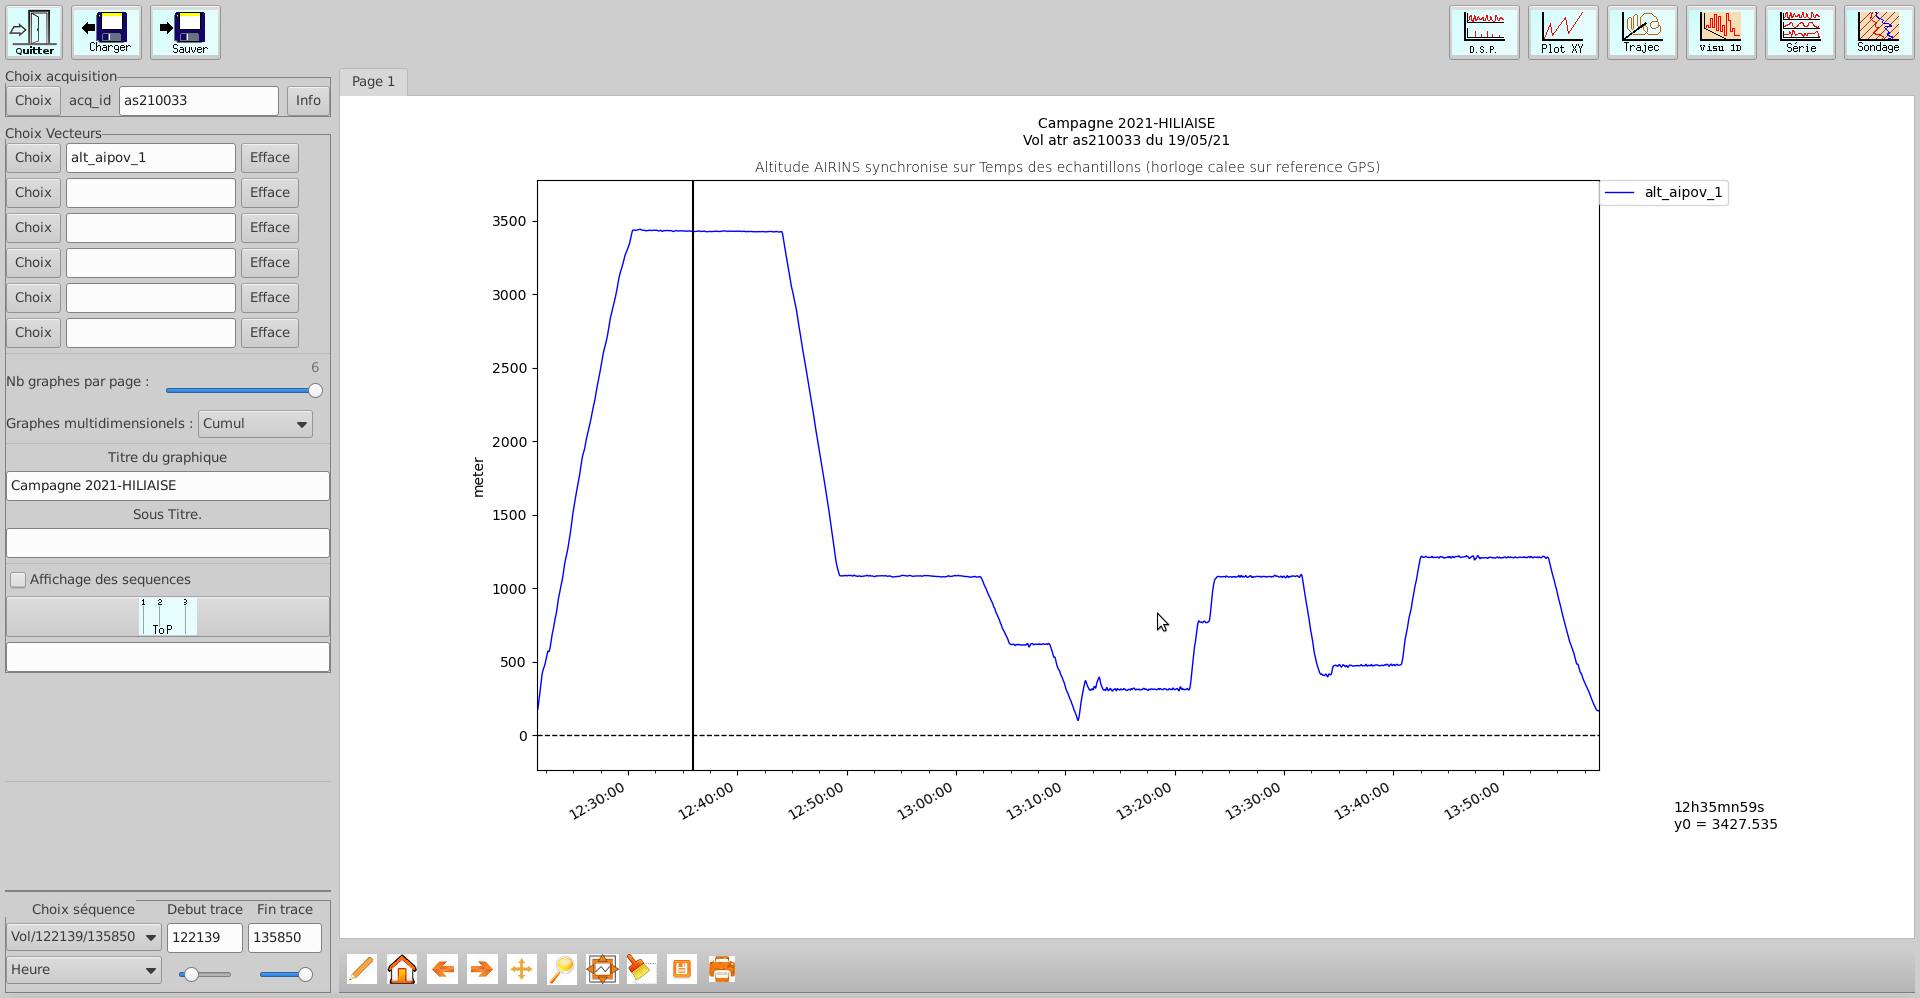
\includegraphics[width=14cm]{images/adp.png}
\end{center}

::: ICI : lorsque Pascal aura installé le manuel utilisateur, ajouter la ligne
Le \textbf{manuel de l'utilisateur} est accessible par le bouton \textbf{Aide}.


\section{\texttt{vista}}
\texttt{vista} (VIsualisation des Séries Temporelles AIDA) permet de
visualiser graphiquement les données d'acquisitions sur toute une période.
Il permet également de créer un fichier de configuration qui pourra être
utilisé pour générer des fichiers Quicklooks en mode non-interactif
("\textit{mode batch}").

\subsection{Lancement}
\texttt{vista} peut être lancé sous \texttt{aito} par l'intermédiaire du bouton
\texttt{vista}
ou en ligne de commande dans un terminal. \\
Lancer la commande \fbox{ \texttt{vista -h} } pour obtenir de l'aide.

\subsection{Présentation}
La page principale de \texttt{vista} comporte plusieurs parties :

\begin{center}
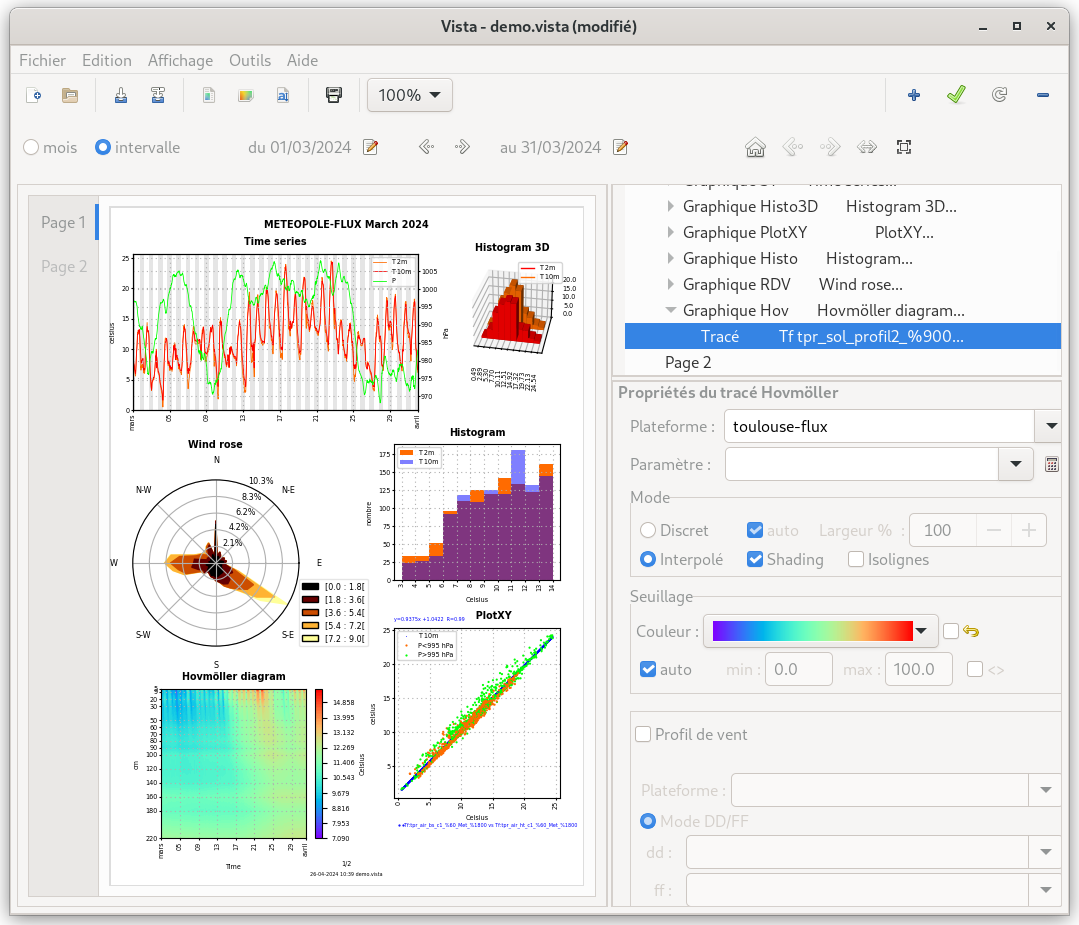
\includegraphics[width=14cm]{images/vista.png}
\end{center}

Le \textbf{manuel de l'utilisateur} est accessible sous l'entrée \textbf{Aide}
du menu principal.


\section{\texttt{gengraphvect.py}}
\texttt{gengraphvect.py} permet de générer le graphe généalogique d'un vecteur.

\subsection{Lancement}
\texttt{gengraphvect.py} peut être lancé sous \texttt{aito} (lorsqu'un vecteur
est sélectionné), par le bouton \texttt{arbre généalogique} de l'onglet
\texttt{données}
ou en ligne de commande dans un terminal. \\
Lancer la commande \fbox{ \texttt{gengraphvect.py -h} } pour obtenir de l'aide.

\medbreak
\textbf{\textit{Note : sous \texttt{aito}, \texttt{gengraphvect.py} est lancé
en mode \texttt{ascendant} avec l'opion de niveau : \texttt{3}}.}

\subsection{Présentation}
L'interface graphique de \texttt{gengraphvect.py} est déportée dans le
programme : \\
\texttt{\path{ihm_genere_graph_geneal_vect.py}} qui doit être lancé en ligne de
commande dans un terminal par la commande :
\fbox{ \texttt{\path{ihm_genere_graph_geneal_vect.py}} }.

\begin{center}
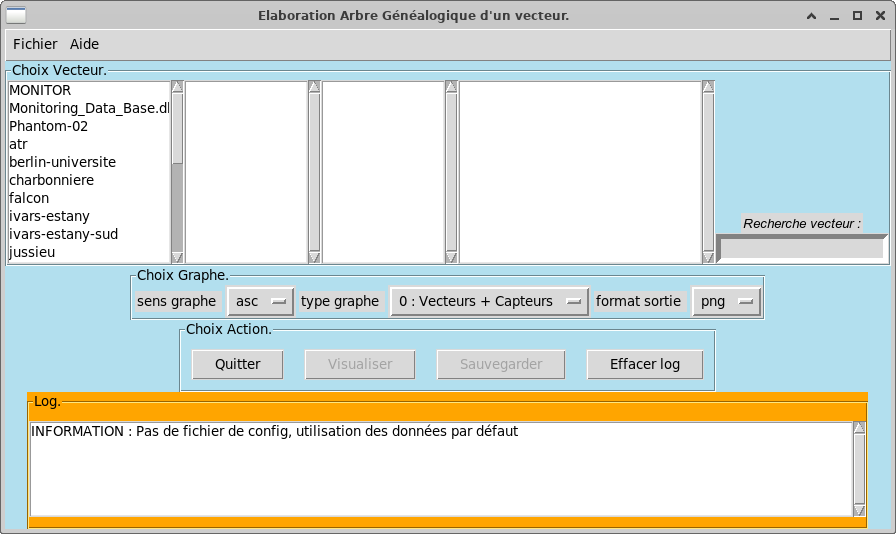
\includegraphics[width=14cm]{images/ihm_genere_graph_geneal_vect.png}
\end{center}

Le \textbf{manuel de l'utilisateur} est accessible sous l'entrée
\textbf{Aide/Doc Utilisateur} du menu principal.


\section{\texttt{genparamvect.py}}
\texttt{genparamvect.py} permet de générer le graphe généalogique d'un vecteur
en suivant un paramètre du header tel que l'unité.

\subsection{Lancement}
\texttt{genparamvect.py} doit ête lancé en ligne de commande un terminal. \\
Lancer la commande \fbox{ \texttt{genparamvect.py -h} } pour obtenir de l'aide.



% Partie 6 : Production de fichiers exportables
\newpage
\part{Production de fichiers exportables}
\label{part:ecriture}
\section{Introduction}
On appelle \textit{fichiers exportables} des fichiers qui vont pouvoir être
relus par d'autres programmes (tableurs, grapheurs) ou transférés dans une
base de données.

\section{Fichiers texte («ASCII»)}
Le programme \texttt{simple\_vivect.py} permet de visualiser un fichier
vecteur en texte («ASCII»)

\subsection{Lancement}
\texttt{simple\_vivect.py} peut être lancé sous \texttt{aito} (lorsqu'un
vecteur est sélectionné), par le bouton \texttt{vivect} de l'onglet
\texttt{données} ou en ligne de commande dans un terminal. \\
Lancer la commande \fbox{\texttt{simple\_vivect.py -h}} pour obtenir de l'aide.

\medbreak
\textbf{\textit{Note : sous \texttt{aito}, le résultat de
\texttt{simple\_vivect.py} est visualisé sous  éditeur \texttt{vi}}}


%%% \section{prod_NASA-AMES-1001.sh}
%%% \section{turbulence}
%%%   \subsection{vec2turb}
%%%   \subsection{check\_tur.py}


\section{Fichiers CVS et nasa-ames-1001}
Le programme \texttt{prod\_csv.py} permet de générer un fichier au format CSV
ou au format nasa-ames-1001 à partir des vecteurs de différentes acquisitions.

\subsection{Lancement}
\texttt{prod\_csv.py} doit être lancé en ligne de commande dans un terminal. \\
Lancer la commande \fbox{\texttt{prod\_csv.py -h}} pour obtenir de l'aide.


\section{Fichiers NetCDF}

\newcommand{\prodcdf}{\textbf{\texttt{prod\_CDF.py}} }
\newcommand{\netcdf}{\texttt{NetCDF} }
\newcommand\myfontsize{\fontsize{9pt}{10pt}\selectfont}

%%%\subsection{\prodcdf}
Le programme \prodcdf convertit un ensemble de
fichiers-vecteurs \textbf{synchronisés sur une même base de temps} d'une même
plateforme en un (ou plusieurs) fichier(s) au format \netcdf.\\

\subsection{Lancement}
\prodcdf doit être lancer en ligne de commande dans un terminal. \\
Pour obtenir de l'aide sur \prodcdf, lancer la commande :
\fbox{\texttt{prod\_CDF.py -h}}

\medbreak
\textbf{\textit{Note : le programme lancé sous \texttt{aito}, onglet
\texttt{Exportation} est : \texttt{prod\_CDF\_histo.py}. \\
Lancer la commande \fbox{\texttt{prod\_CDF\_histo.py -h}} pour obtenir de
l'aide.}
}


\subsection{Manuel d'utilisation}
Par convention, l'extension des fichiers générés est : \texttt{.nc}.

\medbreak
Il utilise plusieurs sources d'information :
\begin{itemize}
\item
  la ligne d'appel
\item
  le fichier de configuration par défaut
\item
  le fichier de configuration
\item
  le fichier AIDA \texttt{plate-formes}
\item
  le fichier de sélection de vecteur
\item
  les fichiers Vecteur AIDA
\item
  les fichiers .INF
\end{itemize}

\medbreak
Il s'appuie sur plusieurs conventions et documentations :
\begin{itemize}
\item
  \texttt{Normalisation\_des\_métadonnées\_NetCDF\_TRAMM\_usage.pdf}
  (la documentation TRAMM)
\item
  \url{http://cfconventions.org/Data/cf-standard-names/current/build/cf-standard-name-table.html}
\item
  \url{https://wiki.esipfed.org/Attribute\_Convention\_for\_Data\_Discovery\_1-3 }
\item
  \url{https://cfconventions.org/Data/cf-conventions/cf-conventions-1.10/cf-conventions.html}
\item
  \url{https://docs.unidata.ucar.edu/udunits/current/}
\end{itemize}


\subsection{Syntaxe de la ligne d'appel}

La syntaxe d'appel de \prodcdf est la suivante :
\medbreak

\fbox{ \myfontsize\texttt{\prodcdf [-h] [-r dir] [-S select\_file] [-v version] -c config\_file prod\_deb prod\_fin} }
\medbreak

avec :
\medbreak

\begin{center}
\tablefirsthead{}
\tablehead{\hline
  \textbf{option} &
  \textbf{défaut} &
  \textbf{commentaire} \\}
\tabletail{\hline}
\tablelasttail{}
  \begin{supertabular}{|p{4.5cm}|p{1.2cm}|p{9cm}|}
\hline
\textbf{option} &
\textbf{défaut} &
\textbf{commentaire} \\
\hline

\texttt{-h} &
&
affichage de l'aide.
\\ \hline

\texttt{-r dir} \smallbreak
\texttt{-{}-rep\_out dir} \smallbreak
\texttt{-o dir} \smallbreak
\texttt{-{}-out\_dir dir} &
\texttt{./} &
nom du repertoire de sortie
\\ \hline

\texttt{-S select\_file} \smallbreak
\texttt{-{}-select select\_file} &
&
chemin du fichier de sélection des vecteurs \smallbreak
pour les paramètres. \smallbreak
voir \nameref{ref:vector_select}
\\ \hline

\texttt{-c config\_file} \smallbreak
\texttt{-{}-config config\_file} &
&
chemin du fichier de configuration.
\\ \hline

\texttt{-v version} \smallbreak
\texttt{-{}-version version} &
\texttt{1} &
numéro de version des fichiers à produire
\\ \hline

prod\_deb \smallbreak
prod\_fin &
&
sous la forme JJMMAAAA : date de début et de fin à traiter. \smallbreak
sous la forme acqid    : premier et dernier acqid à traiter.
\\ \hline

\end{supertabular}
\end{center}

\begin{warning}
  \begin{itemize}
  \item
    La version historique \texttt{prod\_CDF\_histo.py} est lancée si le
    fichier de configuration ne contient pas de section
    \texttt{[DIRECTIVE]} (voir \nameref{ref:configuration}).
  \item
    L'option \texttt{-S\ select} est incompatible avec la configuration
    \texttt{mode\ =\ periode} (voir \nameref{ref:configuration})
  \item
    \textbf{Le numéro de version ne peut être précisé que par cette
    option}.\\
    Il renseigne l'attribut global \texttt{product\_version} du fichier
    \netcdf.\\
    L'option \texttt{product\_version} dans le fichier de configuration
    est ignorée.
  \item
    Le nom du fichier \netcdf généré dépend de différentes options
    fournies. Voir \nameref{ref:nom_NetCDF}.
  \end{itemize}
\end{warning}

\subsection{Configuration par défaut}

Les informations à inscrire dans les fichiers \netcdf qui
ne changent que très rarement pour une équipe peuvent être définies dans
un fichier de configuration par défaut.
\medbreak

Son nom et sa localisation sont :
\texttt{\textbf{\$AIDA\_HOME/profils/\$AIDA\_PROFIL/CDF.defaults}}
\medbreak

Ce fichier est de type INI (voir \nameref{sec:anx_ini}). \\
\medbreak

Il ne contient qu'une seule section : \texttt{[GENERAL]}
\medbreak


\begin{warning}
Les valeurs des options inscrites dans le fichier de configuration écrassent
celles inscrites dans le fichier de configuration par défaut.\\
Ex :

\begin{longtable}[]{@{}lll@{}}
\toprule
\begin{minipage}[b]{0.30\columnwidth}\raggedright
configuration par défaut\strut
\end{minipage} & \begin{minipage}[b]{0.30\columnwidth}\raggedright
configuration\strut
\end{minipage} & \begin{minipage}[b]{0.30\columnwidth}\raggedright
\netcdf\strut
\end{minipage}\tabularnewline
\midrule
\endhead
\begin{minipage}[t]{0.30\columnwidth}\raggedright
processing\_level = L2\strut
\end{minipage} & \begin{minipage}[t]{0.30\columnwidth}\raggedright
processing\_level = L1\strut
\end{minipage} & \begin{minipage}[t]{0.30\columnwidth}\raggedright
:processing\_level = "L1" ;\strut
\end{minipage}\tabularnewline
\bottomrule
\end{longtable}
\end{warning}

\subsubsection{Remarque}

Pour plus de lisibilité du fichier de configuration, les longues valeurs
des options peuvent être enregistrées sur plusieurs lignes (le caractère
de retour à la ligne (\texttt{\textbackslash{}n}) sera inscrit dans le
fichier \netcdf).

Ex :\\
Si le fichier de configuration contient :

\begin{verbatim}
contributor_name = prénom1: nom1: prénom1.nom1@x.fr: institut1;
                   prénom2: nom2: prénom2.nom2@x.fr: institut2;
\end{verbatim}

le fichier \netcdf contiendra :

\begin{verbatim}
string :contributor_name = "prénom1: nom1: prénom1.nom1@x.fr: institut;\nprénom2: [...]
\end{verbatim}

\subsection{Configuration}\label{ref:configuration}

Les informations spécifiques à la génération d'un fichier
\netcdf sont définies dans un fichier de configuration.
\medbreak

L'extension de son nom est préférentiellement \texttt{.ccdf}.
\medbreak

Ce fichier est de type INI (voir \nameref{sec:anx_ini}). \\
\medbreak

Ce fichier est constitué de plusieurs sections :
\medbreak

\begin{itemize}
\item
  une section \texttt{[DIRECTIVES]}\\
  elle rassemble des informations permettant à \prodcdf de
  travailler (en particulier des informations utiles pour générer le nom
  des fichiers \netcdf) ou pour générer la partie
  \textit{dimensions} du fichier \netcdf.
\item
  une section \texttt{[GENERAL]}\\
  on \textbf{n'y trouve que} des informations qui seront inscrites sous
  le même nom dans le fichier \netcdf dans la partie
  \textit{global attributes}.
\item
  une section par paramètre\\
  pour chaque paramètre, on trouve des informations qui seront inscrites
  dans la partie \textit{variables} du fichier \netcdf ou
  dans la partie \textit{dimensions} .
\end{itemize}
\medbreak

Hors la section \texttt{[DIRECTIVES]}, les sections peuvent
également contenir des \textit{options libres} (voir
\nameref{ref:options_libres})

\subsubsection{Section \texttt{[DIRECTIVES]}}

Cette section des \textbf{obligatoire}. \\
Si elle est absente, \prodcdf lancera la version historique :
\texttt{prod\_CDF\_histo.py}\strut

\begin{center}
\tablefirsthead{}
\tablehead{\hline
  \textbf{option} &
  \textbf{nature}

  \textbf{défaut} &
  \textbf{commentaire} &
  \textbf{exemple} \\}
\tabletail{\hline}
\tablelasttail{}
\begin{supertabular}{|p{3.85cm}|p{1.7cm}|p{4.6cm}|p{5.3cm}|}
\hline
\textbf{option} &
\textbf{nature}

\textbf{défaut} &
\textbf{commentaire} &
\textbf{exemple} \\
\hline

prefix &
obligatoire &
utilisé dans la génération du nom du fichier \netcdf \smallbreak
voir \nameref{ref:nom_NetCDF} &
\textit{CNRM\_MTO\_L2A-30min-Mean}\\
\hline

plateforme &
obligatoire &
\textbf{il ne s'agit pas du champ "platform" du fichier \netcdf} mais de la
plateforme AIDA &
\textit{toulouse-flux} \\
\hline

reftime &
obligatoire &
référence temporelle du fichier \netcdf  \smallbreak
\textbf{et des vecteurs à traiter} &
\textit{rft\_time\_REG\_\%1800} \\
\hline

mode &
obligatoire &
periode ou jour ou mobile \smallbreak
voir \nameref{ref:mode} &
\textit{mobile} pour les plateformes mobiles \\
\hline

date\_format &
facultatif \smallbreak
\%Y\%m\%d &
utilisé dans la génération du nom du fichier \netcdf &
\textit{\%Y-\%m-\%d} \\
\hline

replace\_missing\_vector &
facultatif \smallbreak
False &
les données absentes pour une acquisition sont remplacées par Nan &
\textit{True} \\
\hline

datation\_convention &
facultatif \smallbreak
fin &
utilisé pour la création des bornes temporelles &
\textit{debut} \\
\hline

dimensions &
facultatif \smallbreak
Unlimited &
Unlimited ou Limited

champ \texttt{dimensions} du fichier \netcdf &
\textit{Limited} \\
\hline

\end{supertabular}
\end{center}

\begin{warning}
L'absence d'une option obligatoire de la section
\texttt{[DIRECTIVES]} génère l'affichage d'une erreur (\texttt{+++})
et l'arrêt du programme.
\end{warning}

\begin{warning}
Si la référence temporelle de l'un des vecteurs à traiter n'est pas cohérente
avec le vecteur nommé par l'option \texttt{reftime}, la génération
affiche un message d'erreur (\texttt{+++}) et s'arrête.
\end{warning}


\paragraph{Nom du fichier \netcdf} : \label{ref:nom_NetCDF}

Le nom du fichier \netcdf généré dépend :

\begin{itemize}
\item
  des options fournies dans le fichier de configuration par défaut
\item
  des options fournies dans le fichier de configuration
\item
  de la version précisée par l'option -v de la ligne d'appel
\item
  de l'acqid (pour le champ \{acqid\_date\} du mode \texttt{jour})
\item
  de la date de l'acquisition lues dans le fichier .INF (pour le champ
  \{acqid\_date\} du mode \texttt{mobile})
\end{itemize}

\medbreak
Il est construit de la façon suivante, selon les informations positionnées :

\begin{itemize}
\item
  si mode vaut \textbf{jour} : \\
    \{prefix\}\_\{acqid\_date\}\_V\{version\} ou \\
    \{prefix\}\_\{acqid\_date\}\_\{processing\_level\}\_V\{version\}
    \medbreak

\item
  si mode vaut \textbf{periode} : \\
    \{prefix\}\_\{date\_start\}\_\{date\_end\}\_V\{version\} ou \\
    \{prefix\}\_\{date\_start\}\_\{date\_end\}\_\{processing\_level\}\_V\{version\}
    \medbreak

\item
  si mode vaut \textbf{mobile} : \\
    \{prefix\}\_\{acqid\_date\}\_\{acqid\}\_V\{version\} ou \\
    \{prefix\}\_\{acqid\_date\}\_\{acqid\}\_\{processing\_level\}\_V\{version\} \\
\end{itemize}


\paragraph{Option mode} : \label{ref:mode}

L'option \texttt{mode} permet de spécifier le type de fichier
\netcdf à générer.
\medbreak

Cette option peut prendre une des trois valeurs : \texttt{periode},
\texttt{jour}, \texttt{mobile}.

\begin{itemize}
\item
  \texttt{mode = periode} :

    \prodcdf produit un seul fichier \netcdf couvrant la période définie par
    les arguments \texttt{prod\_deb} \texttt{prod\_fin} de la ligne d'appel.

\item
  \texttt{mode = jour} :
    
    \prodcdf produit un fichier \netcdf pour chaque acquisition de la période
    définie par les arguments \texttt{prod\_deb} \texttt{prod\_fin} de la ligne
    d'appel.

\item
  \texttt{mode = mobile} :
    \prodcdf produit un fichier \netcdf de type \textit{Trajectory} pour chaque
    acquisition de la période définie par les arguments \texttt{prod\_deb}
    \texttt{prod\_fin} de la ligne d'appel.
\end{itemize}

\subsubsection{Section \texttt{[GENERAL]}}

Les options \textcolor{orange}{colorées en orange} sont spécifiques au mode
\textcolor{orange}{\texttt{mobile}}.

\begin{center}
\tablefirsthead{}
\tablehead{\hline
  \textbf{option} &
  \textbf{nature}

  \textbf{défaut} &
  \textbf{commentaire} \\}
\tabletail{\hline}
\tablelasttail{}
\begin{supertabular}{|p{4.6cm}|p{4cm}|p{7.5cm}|}
\hline
\textbf{option} &
\textbf{nature}

\textbf{défaut} &
\textbf{commentaire}
\\ \hline

title &
obligatoire &
\\ \hline

summary &
obligatoire &
\\ \hline

Conventions &
obligatoire  \smallbreak
\textit{CF-1.8, ACDD-1.3} &
\\ \hline

keywords &
obligatoire &
devraient être issus de \smallbreak
\url{https://gcmd.earthdata.nasa.gov/KeywordViewer/scheme/all?gtm\_scheme=all}
\\ \hline

keywords\_vocabulary &
obligatoire \smallbreak
\textit{GCMD: }\url{https://gcmd.earthdata.nasa.gov/KeywordViewer/scheme/all?gtm\_scheme=all} &
\\ \hline

data\_policy &
obligatoire \smallbreak
\textit{""} &
il est souhaitable d'indiquer un data\_policy
\\ \hline

processing\_level &
obligatoire \smallbreak
\textit{L2} &
automatique avec fichier .defaults
\\ \hline

source &
facultatif &
cf. documentation TRAMM : \smallbreak
\textit{surface observation, radiosonde, airborne measurements}
\\ \hline

platform &
souhaité si défini sous \smallbreak
\url{https://skosmos.aeris-data.fr/aeris\_pf/en/}
\\ \hline

doi &
obligatoire &
\\ \hline

creator\_name &
obligatoire &
\\ \hline

source\_config &
automatique &
le nom du fichier de configuration
\\ \hline

institution &
souhaitable &
automatique avec fichier .defaults
\\ \hline

creator\_institution &
souhaitable &
automatique avec fichier .defaults
\\ \hline

creator\_email &
souhaitable &
automatique avec fichier .defaults
\\ \hline

contributor\_role &
souhaitable &
cf. documentation TRAMM : \smallbreak
\textit{principalinvestigator resourceprovider contributor}
\textit{owner funder sponsor editor coauthor custodian pointofcontact author}
\textit{originator distributor processor stakeholder}
\textit{collaborator metadatapointofcontact publisher}
\textit{mediator user rightsholder metadatapointofcontact}
\\ \hline

contributor\_name &
souhaitable &
cf. documentation TRAMM : \smallbreak
\textit{prenom:nom:email:institution}
\\ \hline

id &
automatique &
\{prefix\}\_\{processing\_level\}
\\ \hline

project &
souhaitable &
\\ \hline

comment &
souhaitable &
cf. documentation TRAMM
\\ \hline

coordinates &
préférable pour une plateforme mobile &
voir \nameref{ref:geospatial}
\\ \hline

featureType &
automatique \smallbreak
(si l'option `coordinates` est fournie) \textit{Trajectory} &
voir \nameref{ref:featureType}
\\ \hline

history &
souhaitable et \smallbreak
automatique &
\prodcdf ajoute sa ligne de lancement au champ fourni
\\ \hline

date\_created &
automatique &
date et heure d'exécution de \prodcdf
\\ \hline

date\_modified &
automatique &
date et heure d'exécution de \prodcdf
\\ \hline

time\_coverage\_start &
automatique &
première datation
\\ \hline

time\_coverage\_end &
automatique &
dernière datation
\\ \hline

time\_coverage\_resolution &
automatique \smallbreak
PT\{1./freq\_ech\}S &
ex : PT1800.000000S
\\ \hline

geospatial\_lat\_min \smallbreak
geospatial\_lat\_max \smallbreak
geospatial\_lon\_min \smallbreak
geospatial\_lon\_max \smallbreak
\textcolor{orange}{geospatial\_lat\_units} \smallbreak
\textcolor{orange}{geospatial\_lon\_units} \smallbreak
\textcolor{orange}{geospatial\_vertical\_min} \smallbreak
\textcolor{orange}{geospatial\_vertical\_max} \smallbreak
\textcolor{orange}{geospatial\_vertical\_units} \smallbreak
\textcolor{orange}{geospatial\_vertical\_positive} &
automatique &
A partir du fichier plate-formes pour les plateformes fixes. \smallbreak
A partir des vecteurs de l'option \texttt{coordinates} pour les plateformes mobiles. \smallbreak
voir \nameref{ref:geospatial}
\\ \hline

acqid / \textcolor{orange}{flight\_id} &
automatique &
\textcolor{orange}{flight\_id} pour toutes les plateformes mobiles même les voitures...
\\ \hline

\textcolor{orange}{flight\_date} &
automatique &
A partir du fichier \texttt{.inf}.
\\ \hline

\textcolor{orange}{time\_take\_off} &
automatique &
A partir du fichier \texttt{.inf}.
\\ \hline

\textcolor{orange}{time\_landing} &
automatique &
A partir du fichier \texttt{.inf}.
\\ \hline

\end{supertabular}
\end{center}

\begin{warning}
  Les options qui ne sont pas explicitées ci-dessus sont inscrites dans la
  partie \textit{global attributes} du fichier \netcdf.
\end{warning}


\paragraph{Champs \texttt{geospatial}} : \label{ref:geospatial}

S'ils ne sont pas initialisés manuellement dans le fichier de
configuration, la génération des champs \textit{geospatial\_XXX} dans le
fichier \netcdf se fait de la façon suivante :

\begin{itemize}
\item
  pour une plateforme fixe :\\
  les champs \textit{geospatial\_XXX} sont initialisés avec les
  informations trouvées dans le fichier
  \texttt{\$AIDA\_HOME/profils/\$AIDA\_PROFIL/plate-formes} :
\end{itemize}

\begin{verbatim}
  geospatial_lat_min      = geospatial_lat_max      = latitude  de la plateforme
  geospatial_lon_min      = geospatial_lon_max      = longitude de la plateforme
  geospatial_vertical_min = geospatial_vertical_max = altitude de la plateforme
\end{verbatim}

\begin{itemize}
\item
  pour une plateforme mobile :\\

  \begin{itemize}
  \item
    si l'option \texttt{coordinates} est fournie, alors les champs
    \textit{geospatial\_XXX} sont initialisés avec les données trouvées
    dans les fichiers Vecteurs des paramètres de la liste \texttt{coordinatess}.
  \item
    si l'option \texttt{coordinates} n'est pas fournie, \prodcdf
    affiche un warning.\\
    Les champs \textit{geospatial\_XXX} sont initialisés à \texttt{NaN}
    (ils doivent alors être initialisés manuellement dans le fichier de
    configuration).
  \end{itemize}
\end{itemize}


\paragraph{Champs \texttt{featureType}} : \label{ref:featureType}

Les spécificités de traitement liées à des options \texttt{featureType}
autre que \textit{Trajectory} n'ont pas (encore) été étudiées et
implémentées dans \prodcdf. (voir
\url{https://cfconventions.org/Data/cf-conventions/cf-conventions-1.10/cf-conventions.html\#discrete-sampling-geometries})

\subsubsection{Sections \textit{paramètre}}

\begin{center}
\tablefirsthead{}
\tablehead{\hline
  \textbf{option} &
  \textbf{nature} &
  \textbf{commentaire} \\}
\tabletail{\hline}
\tablelasttail{}
\begin{supertabular}{|p{3cm}|p{4cm}|p{9cm}|}
\hline
\textbf{option} &
\textbf{nature} &
\textbf{commentaire} \\
\hline

long\_name &
obligatoire &
pour une variable auxiliaire : \texttt{+modifier} ou \texttt{modifier+} \smallbreak
voir \nameref{ref:variables_auxiliaires}
\\ \hline

origin &
obligatoire &
nom du paramètre AIDA \smallbreak
(nom du vecteur \textbf{sans} son extension)
\\ \hline

ancillary\_variables &
obligatoire \smallbreak
(si des variables auxiliaires existent) &
liste des variables auxiliaires séparées par un espace
\\ \hline

standard\_name &
automatique &
pour une variable auxiliaire : \texttt{+modifier} ou \texttt{modifier+} \smallbreak
voir \nameref{ref:variables_auxiliaires} \smallbreak
voir \nameref{ref:note_standard_name}
\\ \hline

flag\_values \smallbreak
flag\_meanings &
obligatoire \smallbreak
(pour les variables auxiliaires de type \textbf{status\_flag}) &
voir \nameref{ref:variables_auxiliaires}
\\ \hline

units &
facultatif &
voir \nameref{ref:units}
\\ \hline

source &
facultatif &
voir \nameref{ref:source}
\\ \hline

\end{supertabular}
\end{center}

\begin{warning}
  les options qui ne sont pas explicitées ci-dessus sont inscrites dans la
  partie \textit{variables} du fichier \netcdf.
\end{warning}

\paragraph{Note \texttt{standard\_name}} : \label{ref:note_standard_name}

  Il peut arriver que la recherche automatique du \texttt{standard\_name} ne
  fonctionne pas. Dans ce cas, \prodcdf affiche un warning préfixé par
  \texttt{-+-}. Il est alors souhaitable de positionner l'option
  \texttt{standard\_name} dans le fichier de configuration.


\paragraph{Variables auxiliaires} : \label{ref:variables_auxiliaires}

Concernant l'utilisation et la description des variables auxiliaires
selon la norme CF, se reporter à \nameref{ref:annexes}.
\medbreak

Afin de faciliter la saisie du \texttt{long\_name} et du
\texttt{standard\_name} des variables auxiliaires dans le fichier de
configuration, ces 2 options peuvent être données sous les formes :

\begin{itemize}
\item
  \textbf{+\textit{modifier}}
\item
  \textbf{\textit{modifier}+}
\end{itemize}

A la génération du fichier \netcdf, le signe \texttt{+}
(plus) sera remplacé par le \texttt{long\_name} ou le
\texttt{standard\_name} de la \textit{variable principale}. Un espace sera
inséré entre les 2 parties du nom.
\medbreak

\textbf{Note} :

Le mot \textit{modifier} devrait être l'un de ceux décrits dans
la convention CF (voir \nameref{ref:annexes}).
\medbreak

\subparagraph{Exemple d'utilisation} : 

Si le fichier de configuration contient :

\begin{Verbatim}[fontsize=\myfontsize, commandchars=\\\{\}]
[SWD]
long_name           = Downward short wave radiation
origin              = ray_rgd_cnr1_c2_%60_Met_%1800
ancillary_variables = SWD_FLAG


long_name           = \textcolor{red}{+ancillary}
origin              = ctl_SB_invalid_cnr1_Ftp_%1800
standard_name       = \textcolor{blue}{+percentage_of_gap_filled_values}
\end{Verbatim}

sera retranscrit dans le fichier \netcdf sous la forme :

\begin{Verbatim}[fontsize=\myfontsize, commandchars=\\\{\}]
SWD:standard_name = "\textcolor{green}{surface_downwelling_shortwave_flux_in_air}" ;

SWD_FLAG:long_name = "Downward short wave radiation \textcolor{red}{ancillary}" ;
SWD_FLAG:standard_name = "\textcolor{green}{surface_downwelling_shortwave_flux_in_air} \textcolor{blue}{percentage_of_gap_filled_values}" ;
\end{Verbatim}

\begin{warning}
Attention ! \\
Les variables auxiliaires \textbf{ne sont pas toutes de type
\textit{status\_flag}}. Ce type de variable auxiliaire est réservé à des
variables qui ont un nombre fini de valeurs possibles. Leur descritpion
doit donc contenir les 2 options \texttt{flag\_values} et
\texttt{flag\_meanings} (voir \nameref{ref:annexes}).
\end{warning}


\paragraph{Unité d'un paramètre} : \label{ref:units}

L'unité des paramètres est lue dans le fichier Vecteur associé.
Cependant elle peut être positionnée par la configuration de l'option
\texttt{units}.\\
Si l'unité lue ou configurée est \texttt{unitless} (ou pour des raisons
historiques \texttt{unknown} ou \texttt{without}), elle est inscrite dans le
fichier \netcdf avec la valeur : \texttt{1} (standard UDUNITS).


\paragraph{Source d'un paramètre} : \label{ref:source}

Les capteurs sources d'un paramètre sont recherchés automatiquement par
\prodcdf par interrogation l'outil AIDA
\textbf{\texttt{gengraphvect.py}}. Cependant, elle peut être positionnée par la
configuration de l'option \texttt{source} (en particulier si
\texttt{gengraphvect.py} n'arrive pas à touver l'information, ce qui
peut se produire si un vecteur a été copié depuis une autre
acquisition).
\medbreak

Le format préconisé pour l'option \texttt{source} est :\\
\begin{Verbatim}[fontsize=\myfontsize]
fabricant_1 : modèle_1 : numéro_de_série_1; fabricant_2 : modèle_2 : numéro_de_série_2
\end{Verbatim}

Ex :\\

\begin{Verbatim}[fontsize=\myfontsize]
source = Atexis : PT1000 : 0001; Vaisala : HMP110 : L4150552; Vaisala : PTB220 : X2050007
\end{Verbatim}

\subsubsection{Options libres}\label{ref:options_libres}

  Les \textit{options libres} positionnées dans la section
  \texttt{[GENERAL]} du fichier de configuration seront
  retranscrites sans vérification, dans la partie \textit{global
  attributes} du fichier \netcdf.
  \medbreak

  Les \textit{options libres} positionnées dans les sections \textit{paramètre}
  du fichier de configuration seront retranscrites sans vérification, dans
  la partie \textit{variables} du fichier \netcdf.


\paragraph{Format} :

Les \textit{options libres} sont retranscrites sous forme de
\textbf{chaîne de caractères} dans le fichier \netcdf.

Il est cependant possible, pour \textbf{les sections \textit{paramètre}
seulement}, de forcer l'inscription \textbf{au même format} que celui
du vecteur de données. Pour cela, il suffit d'ajouter le mot-clé \texttt{:NUM}
au nom de l'option.
\medbreak

Exemples :

\begin{longtable}[]{@{}ll@{}}
\toprule
\begin{minipage}[b]{0.47\columnwidth}\raggedright
fichier de configuration\strut
\end{minipage} & \begin{minipage}[b]{0.47\columnwidth}\raggedright
fichier \netcdf\strut
\end{minipage}\tabularnewline
\midrule
\endhead
\begin{minipage}[t]{0.47\columnwidth}\raggedright
valid\_min = 0.\strut
\end{minipage} & \begin{minipage}[t]{0.47\columnwidth}\raggedright
valid\_min = "0."\strut
\end{minipage}\tabularnewline
\begin{minipage}[t]{0.47\columnwidth}\raggedright
valid\_min:NUM = 0\strut
\end{minipage} & \begin{minipage}[t]{0.47\columnwidth}\raggedright
valid\_min = 0.f\strut
\end{minipage}\tabularnewline
\begin{minipage}[t]{0.47\columnwidth}\raggedright
valid\_range:NUM = 0., 1000.\strut
\end{minipage} & \begin{minipage}[t]{0.47\columnwidth}\raggedright
valid\_range = 0.f, 1000.f\strut
\end{minipage}\tabularnewline
\bottomrule
\end{longtable}
(les affichages pour la colonne 'fichier \netcdf' sont ceux donnés par
l'outil \texttt{ncdump})
\medbreak

Il est également possible de forcer une inscription \textbf{dans un
autre format numérique} que celui du vecteur de données (bien que ceci
pourrait ne pas avoir beaucoup de sens\ldots\hspace{0pt}). Pour cela, il
suffit d'ajouter \texttt{:fmt} au nom de l'option, avec pour valeur de
\texttt{fmt} une valeur parmi : \texttt{int8}, \texttt{int16},
\texttt{int32}, \texttt{int64}, \texttt{float32}, \texttt{float64}.

Exemples :

\begin{longtable}[]{@{}ll@{}}
\toprule
\begin{minipage}[b]{0.47\columnwidth}\raggedright
fichier de configuration\strut
\end{minipage} & \begin{minipage}[b]{0.47\columnwidth}\raggedright
fichier \netcdf\strut
\end{minipage}\tabularnewline
\midrule
\endhead
\begin{minipage}[t]{0.47\columnwidth}\raggedright
valid\_range:int8 = 0, 2\strut
\end{minipage} & \begin{minipage}[t]{0.47\columnwidth}\raggedright
valid\_range = 0b, 2b ;\strut
\end{minipage}\tabularnewline
\begin{minipage}[t]{0.47\columnwidth}\raggedright
flag\_values:int8 = 0, 1, 2\strut
\end{minipage} & \begin{minipage}[t]{0.47\columnwidth}\raggedright
flag\_values = 0b, 1b, 2b ;\strut
\end{minipage}\tabularnewline
\begin{minipage}[t]{0.47\columnwidth}\raggedright
flag\_meanings = bon, moyen, mauvais\strut
\end{minipage} & \begin{minipage}[t]{0.47\columnwidth}\raggedright
flag\_meanings = "bon, moyen, mauvais" ;\strut
\end{minipage}\tabularnewline
\bottomrule
\end{longtable}
(les affichages pour la colonne 'fichier \netcdf' sont ceux donnés par
l'outil \texttt{ncdump})
\medbreak


\subsection{Sélection de vecteur}\label{ref:vector_select}

La mécanique de \textit{sélection de vecteur} permet de sélectionner le
vecteur (et éventuellement son commentaire assissié) à utiliser pour un
paramètre \textbf{en fonction d'un acqid}.\\
\medbreak

Exemple : utilisation du vecteur d'altitude généré par l'instrument
\textit{aipov} ou par l'instrument \textit{gps} en fonction de l'acqid
traité.
\medbreak

La mise en oeuvre de la mécanique de \textit{sélection de vecteur} se fait
dans un fichier de type INI (voir \nameref{sec:anx_ini}).

\subsubsection{Formalisme}

Chaque section décrit un choix possible.  \\

Chaque section \textbf{doit obligatoirement} contenir un couple d'options
\textbf{\textit{default}} et \textbf{\textit{default\_cmt}} : ces
options seront utilisées s'il n'existe pas de ligne spécifique pour
l'acqid traité. \\

Chaque section peut contenir plusieurs couples d'options :
\begin{itemize}
  \item \textbf{\textit{XXX}} = valeur
  \item \textbf{\textit{XXX\_cmt}} = valeur
\end{itemize}
\medbreak

où \textbf{\textit{XXX}} peut prendre l'une des trois formes suivantes :

\begin{tabular}{|l|p{8cm}|}
\hline
 acqid & un acqid unique
 
 (ex: Tf230001) \\
\hline
 acqid1-acqid2 & une liste d'acqids compris entre acqid1 et acqid2
 
 (ex Tf230001-Tf23005) \\
\hline
 acqid1-* & une liste d'acqids compris entre acqid1 et le dernier acqid à
 traiter
 
 (ex Tf230001-*) \\
\hline
\end{tabular}
\medbreak

Ces options (\textbf{\textit{XXX}} et \textbf{\textit{XXX\_cmt}}) seront
utilisées pour sélectionner les valeurs spécifiques pour
l'acqid ou la liste d'acqids traité(s).
\medbreak

\subsubsection{Utilisation dans le fichier de configuration de \prodcdf}

La syntaxe d'utilisation dans le fichier de configuation de
\prodcdf est la suivante : \\
- pour sélectioner la variable :
  \texttt{\textbf{\textcolor{red}{\$\{section\}}}} \\
- pour sélectioner le commentaire de la variable :
  \texttt{\textbf{\textcolor{red}{\$\{section\_cmt}\}}}
\medbreak

\subsubsection{Exemple}

Fichier de sélection :
\begin{Verbatim}[fontsize=\myfontsize, commandchars=\\\{\}]
[choix_lat]
default      : gps
default_cmt  : le GPS est plus précis dans les sondages que l'AIPOV
fs170012     : aipov
fs170012_cmt : utilisation de l'AIPOV car le GPS est HS
\end{Verbatim}

Fichier de configuration de \prodcdf :
\begin{Verbatim}[fontsize=\myfontsize, commandchars=\\\{\}]
[LAT]
long_name = latitude $\{choix_lat\}
origin    = pos_lat_$\{choix_lat\}_1
comment   = $\{choix_lat_cmt\}
\end{Verbatim}


\subsection{Exemples de fichiers de configuration de \prodcdf}

\newgeometry{margin=1cm}
\begin{landscape}

\subsubsection{Mode \texttt{periode}}

Excécution :

\begin{Verbatim}[fontsize=\myfontsize, commandchars=\\\{\}]
prod_CDF.py -c tests/Tf-AERIS-base.V7.ccdf -S -o /tmp/Tf -v 1 Tf210001 Tf210365
\end{Verbatim}

Extrait du fichier Tf-AERIS-base.V7.ccdf

\begin{Verbatim}[fontsize=\myfontsize, commandchars=\\\{\}]
[DIRECTIVES]
prefix                 = CNRM_MTO_L2A-30min-Mean
plateforme             = toulouse-flux
reftime                = rft_time_REG_%1800
mode                   = periode
date_format            = %Y-%m-%d
replace_missing_vector = True

[GENERAL]
title        = Meteopole-Flux Meteorological Data
summary      = This dataset contains air temperature, humidity at 2 levels...
keywords     = earth science, atmosphere, atmospheric radiation, ...
doi          = https://doi.org/10.25326/44
source       = ground station

creator_name = X Y

contributor_name = X1: Y1: X1.Y1@domain.fr: Institute;
                   X2: Y2: X2.Y2@domain.fr: Institute;
                   X3: Y3: X3.Y3@domain.fr: Institute;

contributor_role = principalinvestigator;
                   resourceprovider;
                   contributor;

...

[SWD]
long_name           = Downward short wave radiation
origin              = ray_rgd_cnr1_c2_%60_Met_%1800
ancillary_variables = SWD_FLAG

[SWD_FLAG]
long_name           = +ancillary
origin              = ctl_flag_invalid_cnr1_Ftp_%1800
standard_name       = +percentage_of_gap_filled_values
...

# Pourcentage de points de visi sur 30 min < 60km OK
[VISI_MEAS_RATE]
long_name           = Rate of visibility measurement in valid measurement range
origin              = opt_pom_dso_tr30_%60_per_%1800
comment             = Rate of measurements in valid (0, 59999 m), measurement range computed during 30 min

# Moyenne harmonique sur 30mn
[VISI_MOYH]
long_name           = Visibility's harmonic mean
origin              = opt_pom_dso_tr30_%60_Moyh_%1800
valid_range:NUM     = 0, 59999
comment             = Harmonic mean of visibility computed during 30 minutes with measurements into valid range (0,  59999 m). If one of the values was out of valid range the result is set to -99
\end{Verbatim}

\subsubsection{Mode \texttt{mobile}}

Excécution :

\begin{Verbatim}[fontsize=\myfontsize, commandchars=\\\{\}]
prod_CDF.py -c tests/prod_g2401m_%60.ccdf -S tests/choix_vecteurs_params -o /tmp/as -v 1 as220024 as220025
\end{Verbatim}

Extrait du fichier tests/prod\_g2401m\_\%60.ccdf

\begin{Verbatim}[fontsize=\myfontsize, commandchars=\\\{\}]
[DIRECTIVES]
prefix     = ACROSSS-2022_SAFIRE-ATR42_SAFIRE_CHEMISTRY-PICARRO_1MN
plateforme = atr
reftime    = rft_time_PICARRO_%60
mode       = mobile


[GENERAL]
title        = ACROSS-2022 data from Picarro instrument G2401-m
summary      = SAFIRE ATR42 Picarro-G2401-m in situ measurements
keywords     = earth science, atmosphere, aircraft, aircraft motion sensor,
               altitude, CH4, CO2, CO
project      = ACROSS-2022
doi          = http://dx.doi.org/10.25326/467

source       = airborne observation
platform     = SAFIRE-ATR42
coordinates  = time LONGITUDE LATITUDE ALTITUDE

creator_name = X1 Y1, X2, Y2
comment      = Warning : Most measurements are not valid before take-off and
               after landing
history      = First version of Picarro-g2401-m data

contributor_name = X3:Y3:X3.Y3@domain.fr;
                   X4:Y4:X4.Y4@domain.fr;
contributor_role = resourceprovider;
                   principalinvestigator;


[LATITUDE]
long_name           = Latitude
#origin              = pos_lat_g2401m_valid_cal_%60
origin              = ${choix_lat}

[LONGITUDE]
long_name           = Longitude
origin              = pos_lon_g2401m_valid_cal_%60

[ALTITUDE]
long_name           = Altitude
origin              = alt_g2401m_valid_cal_%60
standard_name       = altitude

[CH4]
long_name           = CH4 mixing ratio from Picarro instrument G2401-m
origin              = chm_CH4_g2401m_valid_cal_%60
ancillary_variables = CH4_STDEV FLAG_CH4 NB_POINT_CH4

[CH4_STDEV]
long_name           = Standard deviation of CH4 mixing ratio from Picarro instrument G2401-m
origin              = chm_CH4_stdev_g2401m_valid_cal_%60

[NB_POINT_CH4]
long_name           = Number of points used for the calculation CH4 mixing ratio from Picarro instrument G2401-m
origin              = chm_CH4_NbPoints_g2401m_valid_cal_%60

[FLAG_CH4]
long_name           = Flag+
origin              = chm_CH4_flag_g2401m_valid_cal_%60
standard_name       = +status_flag
flag_values         = U, N, O, K, R, H
flag_meanings       = data_correct_before_manual_quality_control data_incorrect_before_manual_quality_control data_correct_after_manual_quality_control data_incorrect_after_manual_quality_control data_correct_after_manual_quality_control_and_backwards_propagation data_incorrect_after_manual_quality_control_and_backwards_propagation

...
\end{Verbatim}


Fichier de sélection passé en argument \texttt{choix\_vecteurs\_params}

\begin{Verbatim}[fontsize=\myfontsize, commandchars=\\\{\}]
# utilisation dans le fichier de configuration de prod_CDF.py :
#   origine = ven_e_${choix_lat}_25
[choix_lat]
default      = pos_lat_g2401m_valid_cal_%60
default_cmt  = test de prod_CDF
fs170012     = aipov
fs170012_cmt = utilisation de l'AIPOV car le GPS est HS
as220025     = pos_lat_XXX_valid_cal_%60
as220025_cmt = validation de XXX
\end{Verbatim}

\subsubsection{Type \texttt{status\_flag}}

Extrait du fichier as\_status\_flag.V1.ccdf

\begin{Verbatim}[fontsize=\myfontsize, commandchars=\\\{\}]
[DIRECTIVES]
prefix     = as_status_flag
plateforme = atr
reftime    = rft_time_PICARRO_%60
mode       = mobile

...

[CH4]
long_name           = CH4 mixing ratio from Picarro instrument G2401-m
origin              = chm_g2401m_valid_cal_%60
ancillary_variables = FLAG_CH4

[FLAG_CH4]
long_name           = Flag+
origin              = chm_flag_g2401m_valid_cal_%60
standard_name       = +status_flag
flag_values         = U, N, O, K, R, H
flag_meanings       = data_correct_before_manual_quality_control data_incorrect_before_manual_quality_control data_correct_after_manual_quality_control data_incorrect_after_manual_quality_control data_correct_after_manual_quality_control_and_backwards_propagation data_incorrect_after_manual_quality_control_and_backwards_propagation
\end{Verbatim}

\end{landscape}
\restoregeometry


\subsection{Annexes NetCDF}\label{ref:annexes}

\subsubsection{Variables auxiliaires}


\paragraph{\texttt{long\_name} et \texttt{standard\_name}} :

Voir :
\url{https://cfconventions.org/Data/cf-conventions/cf-conventions-1.10/cf-conventions.html\#ancillary-data}

Le \texttt{long\_name} et le \texttt{standard\_name} d'une variable
auxiliaire devraient être ceux de sa \textit{variable principale} augmenté
d'un \textbf{modificateur}

Exemple :

\begin{itemize}
\item
  pour la variable \texttt{q}\\
  standard\_name = \textbf{specific\_humidity}\\
  ancillary\_variables = \texttt{q\_error\_limit}
  \texttt{q\_detection\_limit}
\item
  pour la variable auxiliaire \texttt{q\_error\_limit}\\
  standard\_name = \textbf{specific\_humidity} {standard\_error}
\item
  pour la variable auxiliaire \texttt{q\_detection\_limit}\\
  standard\_name = \textbf{specific\_humidity} {detection\_minimum}
\end{itemize}

La description des 4 modificateurs prévus par la convention CF est
présisée sous :\\
\url{https://cfconventions.org/Data/cf-conventions/cf-conventions-1.10/cf-conventions.html\#standard-name-modifiers}.\\
Ces modificateurs sont :

\begin{itemize}
\item
  \textit{detection\_minimum}
\item
  \textit{number\_of\_observations}
\item
  \textit{standard\_error}
\item
  \textit{status\_flag}
\end{itemize}

Le modificateur \textit{status\_flag} est un cas particulier : voir
\nameref{ref:status_flag}


\subparagraph{Attention} :

Cette liste ne couvre pas tout les besoins (ex :
variable auxiliaire précisant le pourcentage de valeurs remplacées). De ce
fait, \prodcdf ne vérifie pas les modificateurs qui lui sont fournis
et \textbf{l'utilisateur peut définir son propre modicateur} sous la
forme de mots séparés par le caractère '\_' (ex :
percentage\_of\_gap\_filled\_values)


\paragraph{\texttt{status\_flag}} : \label{ref:status_flag}

Voir :\\
\url{https://cfconventions.org/Data/cf-conventions/cf-conventions-1.10/cf-conventions.html\#flags}~\\
et\\
\url{https://cfconventions.org/Data/cf-conventions/cf-conventions-1.10/cf-conventions.html\#standard-name-modifiers}

Toutes les variables auxiliaires ne sont pas de type
\textit{status\_flag}.\\
Dans le cas où la variable auxiliaire est vraiment un
\textit{status\_flag}, la section de description de la variable doit
contenir les options \texttt{flag\_values} et \texttt{flag\_meanings} :

\begin{itemize}
\item
  \texttt{flag\_values} est l'ensemble des valeurs possibles de la
  variable.\\
  Les valeurs possibles sont séparées par des virgules.
\item
  \texttt{flag\_meanings} est une description de chacune des valeurs de
  \texttt{flag\_values}.\\
  La descritpion d'une valeur est un ensemble de mots séparés par des
  '\_'.\\
  Les descriptionis sont séparées par des espaces.
\end{itemize}

Exemples :

\begin{verbatim}
flag_values:int8 = 0, 1, 2
flag_meanings    = bon moyen mauvais
\end{verbatim}

\begin{verbatim}
flag_values   = U, N, O, K, R, H
flag_meanings = data_correct_before_manual_quality_control data_incorrect[...]
\end{verbatim}

%%:::::::::: ICI début
%%:::::::::: ICI fin
\begin{warning}

  Pour les variables auxiliaires de type \textit{status\_flag} pour
  lesquelles les valeurs possibles (\textit{flag\_values}) sont des lettres
  (cf. lexemple ci-dessus), l'option \textit{flag\_values} est enregistrée
  par \prodcdf dans le fichier \netcdf sous la forme Python "liste de lettres".
  Cependant certains outils de validation interprètent ce format comme
  "une chaîne de caractères" et peuvent afficher une erreur.
\end{warning}

\subsubsection{Validation des fichiers \netcdf}

Il existe plusieurs outils pour valider les fichiers
\netcdf dont : \url{https://compliance.ioos.us/index.html}

\subsubsection{Visualisation des fichiers \netcdf}

Il existe plusieurs outils de visualisation des fichiers
\netcdf dont :

\begin{itemize}
\item
  ncdump : \textit{dump} d'un fichier \netcdf en texte.
\item
  ncview et panoply : outils graphiques
\end{itemize}





%%%% Partie 6 : production de documentation
%%%\newpage
%%%\part{Documentation des données et traitements effectués}
\label{part:doc}
\section{Introduction}

   L'architecture AIDA est conçue pour traiter la metadonnée
conjointement à la donnée : 
en-tête de fichier vecteur contenant des attributs descriptifs,
méta-données sur les acquisitions regroupées dans fichiers \path{.inf}

    Pour être utilisée, affichée, partagée, cette information
doit être sélectionnée, parcourue, mise en forme. C'est le rôle 
des programmes décrits ici.


\section{mk\_doctrt}
     Qu'il soit une mesure brute ou le résultat d'un
calcul, chaque fichier-vecteur contient dans son en-tête 
des informations sur les conditions de sa production. 

Le programme \texttt{mk\_doctrt} produit un document \LaTeX
décrivant une liste de vecteurs, typiquement le contenu d'un
fichier produit et diffusé.

\texttt{mk\_doctrt} a deux syntaxes d'appel :
\begin{itemize}
\item La première forme consiste en une simple liste d'arguments, qui
doivent être en nombre fixe (3) et dans l'ordre : \lstinline[basicstyle=\ttfamily]{mk_doctrt Acq_id  list_vect AA-EXP}
\item La seconde forme utilise le système usuel des lignes
de commandes, ce qui permet des arguments optionnel, et un ordre qui
n'est pas figé :\\
 \lstinline[basicstyle=\ttfamily]
  {mk_doctrt -a Acq_id -f list_vect -d AA-EXP [-l LL] [-u s|m|h|d|F] }
\end{itemize}

\begin{description}
 \item[Acq\_id] identificateur d'acquisition (6 à 8 caractères). Ex : \texttt{me9814}
 \item[list\_vect] fichier contenant la liste des vecteurs à documenter. Ce
               fichier peut être un fichier de type \texttt{.ofs}.  
               Ce nom sera utilisé comme nom du "dataset".
 \item[AA-EXP] répertoire de campagne contenant la doc dans "notes" (ex : 98-FETCH)
 \item[LL] Code ISO-639-1 de la langue (fr pour français, en pour anglais)
 \item[s|m|h|d|F] unité de la fréquence : F pour Hertz, s pour période en seconde, ...
\end{description}

\section{tab\_camp\_HTML\_v2}

Ce script produit un tableau récapitulatif d'une campagne au format HTML.

Il trouve, parmi les fichiers .inf d'une plate-forme, ceux qui correspondent
à une campagne donnée, et en extrait les lieux et heures
de départ et d'arrivée, ainsi que le thème.


% Partie 7 : utilitaires
\newpage
\part{Utilitaires}
\label{part:utile}
\section{Introduction}
Il existe sous AIDA d'autres outils et utilitaires. Généralement, ils
présentent leur \textit{usage} lorsqu'ils sont lancés, dans un terminal, avec
la seule option \textbf{-h}. Cependant, certains d'entre eux présentent leur
\textit{usage} lorsqu'ils sont lancés sans option (ex : \textit{plt.py}).

Les paragraphes suivants ne documentent que certains de ces outils et
utilitaires. Pour connaitre la liste complète de ces outils et utilitaires,
il suffit de consulter le contenu du répertoire \texttt{\$AIDA\_HOME/bin}.


\section{Création de vecteurs}

\begin{center}
\tablefirsthead{}
\tablehead{\hline
  \textbf{commande} &
  \textbf{rôle} \\}
\tabletail{\hline}
\tablelasttail{}

\begin{supertabular}{|p{6cm}|p{9cm}|}
\hline
\textbf{commande} &
\textbf{rôle}
\\ \hline

\path{cat_vect.py} &
Concatenation de plusieurs vecteurs.
\\ \hline

\path{creer_vect_flag_periode.py} &
Creation d'un vecteur FLAG \path{Int_32} qui vaut la valeur spécifiée en 4eme 
colonne, dans les périodes de temps définies dans le fichier et 0 ailleurs.
\\ \hline

\path{creer_vect_time_sequences.py} &
Utilitaire pour créer des vecteurs \path{rft_tim} et \path{rft_bnds} associés
correspondant à des séquences du fichier \path{.inf} d'un acqid donné.
\\ \hline

\path{recale_vecteur.py} &
Recale un vecteur entre J 00H et J+1 00H sur le principe que la 1ère valeur
de J+1 appartient à J. On ajoute \path{_rec_} avant la fréquence au nom du
vecteur.
\\ \hline

\end{supertabular}
\end{center}


\section{Listes d'acqid}
Les acqids peuvent parfois être donnés sous forme de listes, comme dans les
fichiers de description des campagnes de mesures (voir le document de
référence : \url{refman.pdf}).
Les outils suivants permettent de  travailler avec ces listes :

\begin{center}
\tablefirsthead{}
\tablehead{\hline
  \textbf{commande} &
  \textbf{rôle} \\}
\tabletail{\hline}
\tablelasttail{}

\begin{supertabular}{|p{6cm}|p{9cm}|}
\hline
\textbf{commande} &
\textbf{rôle}
\\ \hline

\path{expand_acqids_list.py} &
Affiche la liste exhaustive des acqids correspondants à la liste compacte
d'acqids passée en argument.
\\ \hline

\path{diff_acqids_list.py} &
Affiche la différence entre 2 listes compactes d'acqids passées en argument.
\\ \hline

\end{supertabular}
\end{center}


\section{Evolution des fichiers de configuration dans le temps}
Les fichiers de configuration des différents outils AIDA peuvent évoluer dans
le temps. La gestion des différentes versions peut être faite grâce à des
fichiers \path{.histo} qui sont analysés par l'outil \path{histo_config.py}
(voir : \ref{sec:histo_config}, page \pageref{sec:histo_config}).

\begin{center}
\tablefirsthead{}
\tablehead{\hline
  \textbf{commande} &
  \textbf{rôle} \\}
\tabletail{\hline}
\tablelasttail{}

\begin{supertabular}{|p{6cm}|p{9cm}|}
\hline
\textbf{commande} &
\textbf{rôle}
\\ \hline

\path{histo_config.py} &
Lit un fichier de type histo et retourne le fichier de config à utiliser pour
le coupleur et la date donnés.
\\ \hline

\end{supertabular}
\end{center}


\section{Petits utilitaires}

\begin{center}
\tablefirsthead{}
\tablehead{\hline
  \textbf{commande} &
  \textbf{rôle} \\}
\tabletail{\hline}
\tablelasttail{}

\begin{supertabular}{|p{6cm}|p{9cm}|}
\hline
\textbf{commande} &
\textbf{rôle}
\\ \hline

\path{doy.py} &
Utilitaire autour des datations de type DOY.
\begin{verbatim}
  doy.py <acqid>
  doy.py <yy0xxx>
  doy.py <yyyy-mm-dd>|<dd/mm/yyyy>
  doy.py <yyyymmdd>
\end{verbatim}
\\ \hline

\path{plt.py} &
Utilitaire autour des noms et abreviations de platefomres.
\begin{verbatim}
  plt.py <abréviation>
  plt.py <au moins 3 caractères>
\end{verbatim}
\\ \hline

\path{Units.py} &
Notation AIDA d'une unité.
\begin{verbatim}
  Units.py <votre unité>
\end{verbatim}
\\ \hline

\end{supertabular}
\end{center}



% Annexes
\newpage
% Annexes
\part{Annexes}
\section{Format de fichier INI}
\label{sec:anx_ini}

  Les fichiers sont divisés en sections.

  Chaque section débutte par un nom écrit entre crochets (\texttt{[]}),
  suivi par des lignes du type : \\
  \texttt{option~=~valeur}.

  Les commentaires sont introduits par le caractère dièse (\texttt{\#}).

  Les noms de section et d'option sont généralement \textit{case-sensitive}
  (''sensible à la casse'').

  Ex :
  \begin{lstlisting}
    # Description du format de fichier INI
    [section_1]
    option_1 = exemple

    [EDITOR]
    Prefered = vi
  \end{lstlisting}


\end{document}
